% Thesis format
\documentclass[11pt, twoside]{book}

%Select needed packages
\usepackage[paperwidth=17cm, paperheight=22.5cm, bottom=2.5cm, right=2.5cm]{geometry}
\usepackage{amssymb,amsmath,amsthm} 
\usepackage[spanish, es-nodecimaldot]{babel}
\usepackage[utf8]{inputenc} 
\usepackage{enumerate}
\usepackage{graphicx}
\usepackage[nottoc]{tocbibind}
\usepackage[pdftex,
            pdfauthor={Alejandro Tarango},
            pdftitle={Interaccion de Flujos Multiples},
            pdfsubject={Astrofísica},
            pdfkeywords={Bowshocks},
            pdfproducer={Latex con hyperref},
            pdfcreator={pdflatex}]{hyperref}
\usepackage{natbib}
%\usepackage[varg]{newtxmath}
%\usepackage{newtxtext}
\usepackage{microtype}
\usepackage{adjustbox}
\usepackage{xcolor}
\usepackage{aas_macros}
\usepackage{fixltx2e}
\usepackage{caption}
\usepackage{booktabs}
\usepackage{siunitx}
\usepackage{pdfpages}
\usepackage{color}
\usepackage{nonumonpart}
\usepackage{pdflscape}
\usepackage{rotating}
\usepackage{hyperref}
%\usepackage[document]{ragged2e}
\usepackage[font=footnotesize]{caption}
\hypersetup{colorlinks=True, linkcolor=blue!50!black, citecolor=black,
  urlcolor=blue!50!black}

\usepackage{etoolbox}
\robustify\bfseries
\robustify\itshape


%% Bold italic
\newcommand\hmmax{0}            % we don't need heavy fonts
\newcommand\bmmax{1}            % reduce use of math alphabets for bold
\usepackage{bm}
\usepackage{fancyhdr}
%\usepackage[fit]{truncate}
\newcommand\thC{\(\theta^1\)\,Ori~C} %Theta 1 C. For further use in any chapter
\newcommand\Ion[2]{\ensuremath{\mathrm{#1\,\scriptstyle #2}}} %Used when naming different ions. Credit: William J. Henney
\newcommand\Nio{\ensuremath{\mathcal{N}}}
\title{Tesis de doctorado\\
\includegraphics[width=0.1\linewidth]{./Figures/tux-development}
}

\author{Jorge Alejandro Tarango Yong}
\DeclareCaptionFormat{cont}{#1 (cont.)#2#3\par}
\begin{document}
\maketitle
\pagestyle{empty}
\begin{center}
\large
\textbf{UNIVERSIDAD NACIONAL AUTÓNOMA DE MÉXICO}

\rule{\linewidth}{0.1pt}

\rule[3mm]{0.7\linewidth}{1pt}

INSTITUTO DE RADIOASTRONOM\'IA Y ASTROF\'ISICA
\\[3\baselineskip]
``Estudio de la Interacción de Flujos Múltiples de Fuentes Astrofísicas, Aplicada
a los Proplyds Clásicos de la Nebulosa de Orión''
\\[2\baselineskip]

T E S I S
\\[2\baselineskip]
PARA OBTENER EL GRADO ACADÉMICO DE

DOCTOR EN CIENCIAS (ASTRONOMÍA)
\\[2\baselineskip]

P R E S E N T A
\\[2\baselineskip]
JORGE ALEJANDRO TARANGO YONG

Director de Tesis: Dr. William J. Henney
\\[2\baselineskip]
\normalsize
\end{center}
\begin{flushright}
Morelia, Michoacán

2017

\end{flushright}

\tableofcontents
\newpage
\section*{\centering Agradecimientos}
\addcontentsline{toc}{section}{\protect\numberline{}Agradecimientos}

% Esta tesis se realizó para obtener el título de doctorado en ciencias (Astronomía). Deseo aprovechar esta sección para hacer agradecimientos a personas y/o instituciones que me ayudaron para que pueda completar este trabajo de manera exitosa.
Primero que nada debo agradecer al Instituto de Radioastronomía y Astrofísica por haberme dado el priviligio de formar parte del Posgrado en Astrofísica para obtener el título de Doctor en Astrofísica. La dedicación, la disciplina y el pensamiento crítico son algunas de las habilidades que adquirí durante la estancia de esta magnífica institución.

En segunda agradezco al Consejo Nacional de Ciencia y Tecnología (CONACyT) por haberme asignado una beca nivel Nacional, del año 2013 al 2017, mi número CVU es 378230.

También quiero agredecer a mi asesor Will por su paciencia, sus buenos consejos y por todo lo que pude aprender de él tanto en la maestría como en el doctorado, y por la oportunidad que me dio de presentar mi trabajo en aquel congreso en Grecia.

A Karin por su amistad y por la ayuda que nos proporcionó durante todo en posgrado. A Rafa también por su amistad y por toda la trayectoria en materia de divulgación que tuve durante mi estancia en el instituto.

Mis padres también tienen una parte especial de mí: ellos me ayudaron cuando terminó el contrato de mi beca CONACyT: de no ser por su ayuda, esta tesis hubiera tomado aún más tiempo terminarla. También sus consejos y su cariño han sido fundamentales para poder llegar a ser quien soy el día de hoy.

Por último y no menos importante, a mi familia: mi amada esposa Betty y mi hija Carmen. Por ellas es por quienes tengo fuerzas todas las mañanas de levantarme y seguir adelante, aunque el resto de mi cuerpo y mi mente me digan lo contrario. A veces parece que no es así, pero nunca estaré arrepentido de que estén a mi lado, y nunca me rendiré para que podamos salir adelante, no importa el tiempo que tome.
\newpage
\section*{\centering Resumen}
\addcontentsline{toc}{section}{\protect\numberline{}Resumen}

Los choques de proa astrofísicos son un resultado común de la interacción de flujos de gas desplazándose a velocidades supersónicas, tales como vientos de estrellas jóvenes o jets de pequeña o grande escala (desde estrellas jóvenes hasta AGNs). Desarrollamos una teoría general para estudiar los efectos de proyección en su forma aparente. Proponemos una nueva clasificación para su forma basándonos en dos parámetros adimensionales medibles a partir de imágenes observacionales: la \textit{planitud} del ápex del choque, y la apertura de las alas, al que llamamos \textit{alatud}. Calculamos la distribución esperada en el diagrama planitud-alatud para modelos físicos y geométricos simples: cuádricas de revolución, choques cantoides, ancantoides y wilkinoides. Por último, comparamos estos modelos con observaciones de los choques de proa observados en las proximidades del Trapecio, en la Gran Nebulosa de Orión.


\section*{\centering Abstract}
\addcontentsline{toc}{section}{\protect\numberline{}Abstract}

  Astrophysical bow shocks are a common result of the interaction of supersonic gas flows, such as winds generated by young stars or jets from small to large scale (from young stars to AGNs). We develop a general theory for the projection effects on the apparent shape. We propose a new classification scheme based in two dimensionless parameters that can be estimated from observational images: the \textit{planitude} of the bow's apex and the openess of the wings, which we term \textit{alatude}. We calculate the expected distribution in the planitude-alatude diagram for simple geometrical and physical models: quadrics of revolution, cantoids, ancantoids and wilkinoids. Finally, we compare these models with observations of the bow shocks observed near the Trapezium, in the Great Orion Nebula.

\newpage
\section*{\centering Prefacio}
\addcontentsline{toc}{section}{\protect\numberline{}Prefacio}

Los choques de proa se producen cuando un flujo de gas se mueve a velocidades supersónicas e interactúa con el medio que lo rodea. Aparecen en diferentes escenarios astrofísicos, como mencionaremos más adelante.

En trabajos anteriores se intentó obtener información relevante acerca de las propiedades de choques de proa dentro de la Nebulosa de Orión producidos por proplyds basándose en mediciones de su forma aparente \citep{Robberto:2005}, sin embargo, las mediciones de algunos de estos choques no concordaban con el modelo teórico utilizado para obtener dicha información. La motivación inicial de este trabajo consistía en extender el modelo de aproximación de capa delgada para la interacción de dos vientos \citep{Canto:1996} para incluir el escenario donde el viento interior deja de ser isotrópico, esperando que las mediciones de la forma del choque producido por esta clase de vientos ajuste mejor a la forma de los choques de proa restantes en la Nebulosa de Orión.

Esta tesis está estructurada de la siguiente manera: en el capítulo \ref{chap:ONC} mencionamos algunas características generales de la Nebulosa de Orión, la región \Ion{H}{II} por excelencia para estudiar el escenario de la formación estelar y donde se han encontrado una gran variedad de objetos y fenómenos astrofísicos de gran interés, así como el modelo aceptado actualmente de la formación de los proplyds, que son los que producen los choques de proa observados en las Nebulosa de Orión, y muy probablemente en otras regiones \Ion{H}{II}. En el capítulo \ref{chap:bow-shocks} se explican diferentes escenarios donde se pueden formar choques de proa. En el capítulo \ref{chap:Modelo-generico} se explican conceptos fundamentales que nos serán de gran utilidad para entender los modelos de interacción de vientos de los que obtendermos la forma de los choques de proa, tales como los ``radios característicos'', que son los parámetros medibles con los que determinaremos la forma de los choques de proa: la ``planitud'', que nos indica qué tan plano es el choque de proa en la nariz o ``ápex'', y la ``alatud'', que nos indica qué tanto se abren las alas del choque. También explicaremos como para un choque geométricamente delgado y ópticamente delgado su orientación respecto al plano del cielo influye en la forma que observamos, y lo ejemplificamos con las formas más simples (aunque no necesariamente plausibles físicamente): las cuádricas de revolución. El capítulo \ref{chap:hipersonica} explica a detalle el modelo de capa delgada de \citet{Canto:1996} en el que nos basamos para modelar la forma de los choques de proa, y explicamos la extensión a este modelo que realizamos. Asimismo mostramos cómo sería su forma aparente si su eje de simetría no estuviera en el plano del cielo. En el capítulo \ref{chap:proplyds} aplicamos los resultados de los capítulos anteriores a los choques de proa formados por los proplyds de la Nebulosa de Orión. Por último, en el capítulo \ref{chap:conclusions} enumeramos las conclusiones finales de este trabajo.

Esta tesis también cuenta con apéndices donde explicamos a detalle conceptos importantes para esta tesis: los apéndices \ref{app:HII}-\ref{app:shocks} explican el modelo actual de las regiones \Ion{H}{II} y la física detrás de los choques y Frentes de Ionización, que nos ayudará a entender cómo se forma el viento fotoevaporado e ionizado de un proplyd. El apéndice \ref{app:math-curvature-radius} contiene el procedimento matemático con el que se define y se calcula el Radio de Curvatura (uno de nuestros radios característicos) para una curva genérica, siempre y cuando sea continua y derivable. El apéndice \ref{app:derivation-radii} explicamos de manera detallada cómo se obtienen las ecuaciones para calcular los radios característicos en el modelo de capa delgada. Por último, en el apéndice \ref{app:article} mostrmos el artículo en que se basa gran parte de esta tesis (parte del capítulo \ref{chap:bow-shocks} y los capítulos \ref{chap:Modelo-generico} - \ref{chap:hipersonica}), actualmente publicado (el capítulo \ref{chap:proplyds} se basa en un artículo que aún no está terminado y probablemente los resultados presentados aquí serán incluídos).

\begin{figure}
  \centering
  \includegraphics[width=0.4\linewidth]{./Figures/helping}
  \caption*{Esta tesis no la hice solo, recibí un poco de ayuda.}
\end{figure}


\newpage

  

\pagestyle{fancy}
\fancyhf{}
\fancyhead[LE]{\footnotesize \thepage \quad\leftmark}
\fancyhead[RO]{\footnotesize \rightmark \quad\thepage}
\chapter[La Nebulosa de Orión]{La Nebulosa de Orión: La Fotoevaporación de Discos Protoplanetarios como una Forma de Feedback Estelar}
\thispagestyle{empty}
\label{chap:ONC}
\section{Características Generales}
\begin{figure*}
  \centering
 % \begin{tabular}{cc}
    \includegraphics[width=\linewidth]{./Figures/orion-HST-NRAO} 
 % \end{tabular}
    \caption{Izquierda: La nebulosa de Orion tomada con el Telescopio Espacial Hubble (hubblesite.org). Derecha: La Nebulosa de Orión observada por el VLA en la banda L ($\lambda = \SI{20}{cm}$, $\nu = \SI{1.4}{GHz}$, \citet{Yusef:1990}). La región observada en esta imagen corresponde aproximadamente al recuadro mostrado en la imagen de la izquierda. Créditos: NASA, ESA, NRAO.}
    \label{fig:orion-pretty}
\end{figure*}

El cúmulo de las Nebulosa de Orión (ONC por sus siglas en inglés, figura \ref{fig:orion-pretty}), ubicada a $\sim \SI{414}{pc}$ \citep{Menten:2007}, es probablemente la región \Ion{H}{II} mejor estudiada del cielo (ver apéndice \ref{app:HII}). Forma parte de la nube molecular gigante de Orión, de donde se distinguen dos sub-unidades, llamadas Orión A y Orión B. ONC forma parte de Orión A. El cúmulo de estrellas masivas que se formó y que es responsable de la región \Ion{H}{II} se conoce como asociación OB Ori Id, cuyos miembros más prominentes son un grupo de cuatro estrellas conocidas como el ``Trapecio''. La más masiva de éstas es \thC{}, de clasificación espectral O6 aproximadamente (ver tabla \ref{tab:ionizing-radiation}), tiene una luminosidad de \SI{4e5}{L_\odot} y una temperatura de \SI{4e4}{K}. Cuando la región \Ion{H}{II} se encuentra embebida en el gas molecular, no puede ser visible en el rango óptico del espectro. En el caso de ONC, que se ubica cerca del borde de la nube molecular Orion A, el gas ionizado caliente, que posee una presión mayor que el gas molecular frío, se escapa hacia el gas adyacente de la nube molecular en forma de ``flujo de champaña'', de modo que el gas ionizado se acerca a nosotros a una velocidad de $\sim \SI{3}{km.s^{-1}}$, mientras que ONC se aleja a una velocidad de $\sim \SI{10}{km.s^{-1}}$ (\citet{Stahler:2004}, ver figura \ref{fig:champagne}). De esta manera el gas ionizado puede ser visible por medio de diferentes líneas espectrales, tanto de hidrógeno como de otros elementos. 

\begin{figure}
  \centering
  \begin{tabular}{lr}
    \includegraphics[width=0.4\linewidth]{./Figures/champagne} &
    \includegraphics[width=0.5\linewidth]{./Figures/H85-alpha}
    \end{tabular}
  \caption{Izquierda: Representación esquemática de la Asociación Ori Id y su ubicación dentro de la nube molecular gigante Orión A. La región BN-KL es una región de formación estelar muy activa donde se observan entre otras cosas, máseres de agua, SiO y flujos moleculares \citep{Stahler:2004}. Derecha: Línea espectral \Ion{H85}{\alpha} de hidrógeno de ONC. El eje horizontal corresponde a la frecuencia en MHz, mientras que el eje vertical representa la temperatura de antena. El espectro muestra un corrimiento al azul que muesta que el gas se acerca a una velocidad de $\sim \SI{3}{km.s^{-1}}$ \citep{Stahler:2004, Churchwell:1970}}
  \label{fig:champagne}
\end{figure}

\section{Proplyds}
\subsection{Descubrimiento}
Observaciones en óptico de la región del Trapecio en filtros de banda angosta de diferentes líneas de emisión tales como \Ion{H}{\alpha}, \Ion{H}{\beta}, [\Ion{O}{III}], [\Ion{N}{II}], [\Ion{S}{II}] y continuo, revelaron la existencia de objetos puntuales visibles notablemente en líneas de alta ionización (\Ion{H}{\alpha}, \Ion{H}{\beta} y [\Ion{O}{III}]) que fueron inicialmente denominados como ``condensaciones nebulares'' \citep{Laques:1979}. Hasta ese momento no se sabía con certeza si esas ``condensaciones nebulares'' eran en realidad condensaciones nebulares (regiones donde la densidad de la nebulosa es inusualmente alta o bien esferas de gas molecular cuya envolvente fue ionizada y que la radiación de la estrella central la está ``erosionando'') o si se trataba de protoestrellas de baja masa cuyo disco protoplanetario estaba siendo fotoevaporado por la estrella central \citep{churchwell:1987}. No fue sino hasta que se contó con observaciones de alta resolución con el Telescopio Espacial Hubble (HST) que se se pudo determinar la verdadera naturaleza de estos objetos \citep{ODell:1993} y la razón por la que se les denominó ``proplyds'' (PROtoPLanetarY DiskS). A su vez se encontraron por primera vez arcos delgados y otras estructuras de gran interés.

\subsection{¿Qué es un proplyd? Breve introducción \citep{Johnstone:1998}}
\label{sec:prop-Johnstone}

Las imágenes del HST de la Nebulosa de Orión mostraron imágenes de discos alrededor de estrellas jóvenes de baja masa. Algunos se ven como siluetas oscuras que contrastan con la nebulosa, y otros casos son visibles en líneas de emisión de líneas de alta ionización. Un proplyd típico tiene forma cometaria, con una cabeza brillante que apunta hacia la fuente de radiación ionizante, y una cola que se extiende en dirección contraria a ésta, (ver figura \ref{fig:prop-shape}). La explicación a esta forma es que se trata de estrellas T-Tauri que quedaron embebidas por la región \Ion{H}{II} en expansión y el disco protoplanetario está siendo fotoevaporado por la radiación ionizante de una estrella masiva (\thC{} en caso de la Nebulosa de Orión), la cabeza es un frente de ionización cuyo radio escala como $R_{\mathrm{IF}} \propto D^{2/3}$, donde $D$ es la distancia a la estrella masiva. La forma de la cola se debe a radiación  difusa, producto de dispersión por polvo y por recombinaciones. \citet{churchwell:1987} ya había notado que la tasa de pérdida de masa observada en el gas ionizado implicaba que la fuente de este gas debía oscurecer a la protoestrella huésped, a menos que proviniera de un disco circunestelar. De la emisión de radio observada, se estima que la densidad electrónica máxima en el IF es de $n_e \sim \SI{e6}{cm^{-3}}$ y la tasa de pérdida de masa es de $\dot{M} \sim \SI{e-7}{M_\odot.yr^{-1}}$.

\begin{figure}
  \centering
  \includegraphics[width=0.8\linewidth]{./Figures/Johnstone-shape}
  \caption{Representación esquemática de la formación de un frente de ionización hemisférico y de una cola de gas fotoevaporado detrás del disco en proceso de fotoevaporación \citep{Johnstone:1998}. La línea gruesa exterior representa la interfaz donde existe equilibrio entre ionizaciones y recombinaciones en el flujo fotoevaporado. $r_{\mathrm{IF}}$ y $r_w$ representan el radio del frente de ionización en las direcciones de los ejes $x$ e $y$, respectivamente. $I_y$ representa el campo de radiación difusa. Por detrás del disco, la radiación difusa calienta el gas del disco provocando otro flujo fotoevaporado. $\Delta y$ es la diferencia entre la forma actual del frente de ionización por detrás del disco y una forma cilíndrica, y determina la forma de la cola. En esta interfaz debe de haber balance entre ionizaciones provocadas por el flujo $F_y \simeq \pi I_y$ y recombinaciones en el flujo fotoevaporado, y como la densidad de este flujo disminuye al alejarse del disco a lo largo del eje $x$, entonces la zona donde se da el equilibrio de ionización ocurre cada vez más cerca del eje $x$. \citet{Johnstone:1998} muestra que la forma de la cola es tal que $\Delta y \propto x^4$, donde $x$ es la distancia al disco a lo largo del eje $x$. Por otro lado, también se muestra que la cola termina cuando $\Delta y = r_w$ y esta condición se da cuando $x \sim 3 r_w$.} %como que el flujo de radiación $I_y$ es capaz de penetrar más cerca del eje $x$ conforme uno se aleja del disco, donde el flujo fotoevaporado es menos denso.}
    \label{fig:prop-shape}
\end{figure}


\subsection{Mecanismos de fotoevaporación \citep{Johnstone:1998}}
\label{sec:photoevaporation}

El principal mecanismo de fotoevaporación es el campo de radiación de la estrella central, en la parte ultravioleta del espectro electromagnético. Según la masa de la estrella central, podemos tener dos clases de flujo radiativo: Dominado por el ultravioleta lejano (FUV, $h\nu < \SI{13.6}{eV}$) o dominado por el ultravioleta extremo (EUV, $h\nu \geq \SI{13.6}{eV}$). En general, el FUV se encarga de disociar moléculas y de calentar el gas de la región de fotodisociación (PDR) hasta temperaturas de \SI{100}{} - \SI{1000}{K}, mientras que el EUV puede ionizar el gas y elevar su temperatura hasta \SI{e4}{K}. El EUV no puede atravesar el frente de ionización (IF) pero el FUV sí. Inicialmente la forma del disco impone una geometría cilíndrica en el flujo fotoevaporado, pero eventualmente los gradientes de presión tornan esta geometría en esférica, como se muestra en la figura \ref{fig:flux-geometry}.

\begin{figure}
  \centering
  \includegraphics[width=0.7\linewidth]{./Figures/Johnstone-1}
  \caption{Geometría del flujo fotoevaporado de un disco protoplanetario de radio $r_d$ bajo un flujo de fotones ultravioleta provenientes de una fuente puntual lejana. Inicialmente el disco impone una geometría cilíndrica para el flujo, pero los gradientes de presíon en el ambiente convierten rápidamente la geometría del flujo en esférica. El gas que se encuentra a distancias menores a $r_g$ de la estrella central (ecuación \ref{eq:grav-radius}) es retenido por la gravedad de ésta \citep{Johnstone:1998}.}
  \label{fig:flux-geometry}
\end{figure}

En el caso de que el flujo sea dominado por el EUV, la presión térmica del flujo fotoevaporado es determinada por la fotoionización, la PDR producida por el FUV es delgada. El gas calentado por el FUV se mueve de manera subsónica ($v_I \propto r^{-2}$) hasta llegar al IF, donde alcanza una velocidad de \SI{0.5}{km.s^{-1}} y la tasa de pérdida de masa depende de la tasa de ionización inducida por el EUV.

Si el flujo está dominado por el FUV, la presión térmica depende del calentamiento por el FUV. El gas tibio se expande como un viento que empuja el IF lejos del disco que alcanza velocidades supersónicas, pero luego atraviesa un choque isotérmico que lo desacelera y llega al frente de ionizacion a \SI{0.5}{km.s^{-1}}. La tasa de pérdida de masa la determina la temperatura de la PDR, el flujo FUV y la opacidad del polvo a las longitudes de onda del FUV. Este caso y el anterior se muestran en la figura \ref{fig:EUV-FUV-IF}.

Las ecuaciones de continuidad de la masa y el momento restringen la velocidad del flujo neutro antes de alcanzar el IF. Mas allá de éste, la presión del gas hace que éste se expanda a velocidades del orden de una a dos veces la velocidad del sonido, que es de $c_{\mathrm{I}} \sim \SI{3}{km.s^{-1}}$ para el gas neutro, y de $c_{\mathrm{II}} \sim \SI{10}{km.s^{-1}}$ para el gas ionizado. Para el gas neutro dentro del IF hay dos posibles soluciones: si el gas neutro es supersónico entonces el IF será de baja densidad (Tipo R) con bajo contraste de densidad entre gas neutro y gas ionizado. O si el gas neutro es subsónico se formará un IF tipo D con un gran contraste de densidad entre el gas neutro y el gas ionizado. Sin embargo, ya mostramos que sin importar qué tipo de radiación domina la fotoevaporación, el gas neutro permanece a velocidades subsónicas al llegar al IF (figura \ref{fig:EUV-FUV-IF}), por lo que dicho frente será tipo D.

\begin{figure}
  \centering
    \begin{tabular}{cc}
      \includegraphics[width=0.5\linewidth]{./Figures/Johnstone-2} &
      \includegraphics[width=0.5\linewidth]{./Figures/Johnstone-3}
    \end{tabular}
    \caption{Representación esquemática de las regiones del flujo fotoevaporado de un proplyd. Izquierda: Cuando el flujo es dominado por el FUV, se acelera a velocidades supersónicas pero atraviesa un choque isotérmico que lo desacelera a velociades subsónicas. Derecha: Flujo dominado por EUV, que llega a velocidades subsónicas al frente de ionización \citep{Johnstone:1998}.}
    \label{fig:EUV-FUV-IF}
  \end{figure}
  
  
Sin importar el tipo de mecanismo de fotoevaporación dominante, el flujo fotoevaporado existe solo si la presión térmica supera a la gravedad de la protoestrella. Entonces, el flujo fotoevaporado solo existe a partir de un radio crítico $r_g$, donde este radio se estima a partir del balance entre la energía necesaria para escapar de una órbita kepleriana y la energía térmica:
\begin{align}
  r_g = \frac{GM_*}{c^2} \label{eq:grav-radius}
\end{align}
Donde $M_*$ es la masa de la protoestrella y $c$ es la velocidad del sonido del gas. Para las protoestrellas típicas del Trapecio la masa típica es de
$M_* = \SI{0.2}{M_\odot}$. Utilizando las velocidades del sonido para el gas neutro e ionizado, encontramos que el radio gravitacional para un flujo dominado por el EUV es de $r_{\mathrm{gII}} \sim \SI{2}{AU}$ y para un flujo dominado por el FUV es de $r_{\mathrm{gI}} \sim \SI{20}{AU}$.

\chapter[Choques de Proa]{Choques de Proa en el Medio Interestelar}
\label{chap:bow-shocks}
\thispagestyle{empty}

En general, un choque de proa se forma cuando un fluido interactua con un objeto moviéndose a velocidades supersónicas. A continuación enumeramos algunos ejemplos astrofísicos que se pueden encontrar en el medio interestelar:

\begin{itemize}
\item Superficies de trabajo de jets
\item Interacción de magnetósfera con el viento solar
\item Choques de proa estelares
  \begin{itemize}
  \item Estrellas AGB
  \item Estrellas O
  \item \textbf{Proplyds}
  \item Estrellas T Tauri
  \item Estrellas de Neutrones
  \end{itemize}
\end{itemize}

La morfología general de un choque de proa se ilustra en la figura \ref{fig:terminology}. La región donde la distancia entre el choque y la estrella (en el caso de un choque de proa \textit{estelar}) es la mínima, se denomina cabeza o \textit{ápex}, mientras que las regiones más alejadas son denominadas las \textit{alas}. En el caso ideal los choques de proa son cilíndricamente simétricos.

\begin{figure}
  \centering
  \includegraphics[width=0.5\linewidth]{./Figures/bow-terminology}
  \caption{Terminología de un choque de Proa \textit{estelar}.}
  \label{fig:terminology}
\end{figure}

\section{Proplyds}
Observaciones en mediano infrarrojo y en líneas de emisión de \Ion{H}{\alpha} y [\Ion{O}{III}] (\citet{Robberto:2005, Bally:1998, Bally:2000}, ver figura \ref{fig:prop-bally-robberto}) muestran de manera clara la presencia de arcos que rodean varios proplyds y otros objetos en la ON cerca y lejos de la región del Trapecio. \citet{Hayward:1994} abren por primera vez la discusión acerca de la naturaleza de estos arcos (enfocándose en la región del Trapecio), sugiriendo que la presión de radiación y el viento estelar de \thC{} interactúan con el flujo de gas proveniente de cada proplyd individual.

\begin{figure}
  \centering
  \includegraphics[width=0.7\linewidth]{./Figures/Orion_Robberto}
  \caption[La región del Trapecio]{La región del trapecio en \SI{10}{\mu m}. \thC{} es la fuente débil al centro de la imagen. Dentro de este campo además se encuentran los proplyds LV1-LV5 con sus respectivos arcos. Al noreste se encuentra una fuente extensa llamada la Nebulosa Ney Allen (NA). El norte es encuentra hacia arriba y el este a la izquierda. El tamaño del campo es de aproximadamente $1' \times 1'$ \citep{Robberto:2005}.}
  \label{fig:prop-bally-robberto}
\end{figure}

\begin{figure}
  \centering
  \ContinuedFloat
  \captionsetup{list=off,format=cont}
  \includegraphics[width=0.7\linewidth]{./Figures/bally-trapezium}
  \caption{La región del trapecio en mosaico de colores con imágenes de la Cámara Planetaria de Campo Ancho 2 (WPC2) del ciclo 4 del Telescopio Espacial Hubble (HST). El color rojo corresponde al [\Ion{N}{II}], el verde al \Ion{H}{\alpha} y el azul es [\Ion{O}{III}] \citep{Bally:1998}.}
  \label{fig:prop-bally-robberto-2}
\end{figure}


Asimismo, en \citet{Robberto:2005} se hicieron mediciones de la forma de estos arcos, utlizando el radio aparente en el ápex $R_0/D$ y el radio perpendicular a éste $R_{90}/D$ (la alatud en este trabajo, excepto que normalizada con la distancia $D$ a \thC{}, ver \S \ref{sec:char-rad}) para los proplyds LV1-LV5 y la nebulosa Ney-Allen, y los compararon con el modelo de capa delgada \citep{Canto:1996} (figura \ref{fig:Robberto}). Encontraron que aunque los proplyds LV1, LV4 y posiblemente LV5 ajustan a dicho modelo, pero el resto se aleja mucho de las curvas teóricas. Ésto no se puede atribuir a las limitaciones de la aproximación algebraica hecha por \citet{Canto:1996}, debido a que aun con todas las simplificaciones que conlleva, ajusta bien con modelos hidrodinámicos más complejos (ver por ejemplo \citet{Garcia-Arredondo:2001}, figura \ref{fig:GA-simulation}). El trabajo de \citet{Robberto:2005} es en parte la inspiración para esta tesis, ya que para explicar la discrepancia en la figura \ref{fig:Robberto} con los proplyds restantes nos llevó a extender el modelo de \citet{Canto:1996} al caso donde el viento interior no es isotrópico. En la figura \ref{fig:generic-bowshock} se explica el modelo general para explicar éstos choques de proa: el flujo fotoevaporado de un proplyd, ya sea isotrópico o anisotrópico, interactúa con el viento estelar de \thC{}, formando dos choques separados por una discontinuidad de contacto. El frente de ionización del proplyd es tipo D (ver \S \ref{sec:photoevaporation}), por lo que la velocidad del flujo fotoevaporado es cercano a la velocidad del sonido y se acelera máximo hasta $M\sim 3$, donde $M\equiv v_w/c_s$ es el número de Mach, $v_w$ es la velocidad del flujo y $c_s$ es la velocidad del sonido. Y la densidad electrónica del flujo fotoevaporado es de $n_e\sim \SI{e6}{cm^{-3}}$ (ver \S \ref{sec:prop-Johnstone}). Por otro lado, el viento de \thC{} ha alcanzado su velocidad terminal, que es de $M > 100$ con una tasa de pérdida de masa de $\dot{M} \simeq \SI{4e-7}{M_\odot.yr^{-1}}$ \citep{Gagne:2005}. Bajo estas condiciones, el choque exterior es poco denso y extenso y el choque interior es más denso y angosto. Por tanto, el enfriamiento en el choque interior es más eficiente y consideramos que este choque es radiativo mientras que el choque exterior no.

\begin{figure}
  \centering
  \includegraphics[width=0.9\linewidth]{./Figures/robberto}
  \caption[Comparación entre $R_{90}/D$ y $R_0/D$ por \citet{Robberto:2005}]{Comparación entre los radios característicos aparentes $R_{90}/D$ y $R_0/D$ para los proplyds LV1-LV5 y para la Nebulosa Ney-Allen y las soluciones al modelo de capa delgada de \citep{Canto:1996}. Las mediciones de los radios característicos de los proplyds se muestran con puntos y sus respectivas incertidumbres. Las soluciones al modelo de capa delgada se muestran con diametes abiertos unidos con línea continua o de puntos, y cada curva representa un valor diferente para el cociente de las tasas de momentos del viento del flujo fotoevaporado del proplyd al viento estelar de \thC{}, denotado por $\beta$ (definido en la \S \ref{sec:fundamental-parameters}, ecuación \ref{eq:beta-def}). Dichos valores, de izquierda a derecha son $\beta=[0.001, 0.002, 0.004, 0.01, 0.02, 0.1]$. Por otro lado, a lo largo de una misma curva varía la orientación del choque respecto al plano del cielo, medida por un ángulo llamado \textit{inclinación}, denotado como $\theta$ en esta figura, pero en este trabajo se denota con $i$ (ver \S \ref{sec:projection})) y que en esta figura incrementa en intervalos de $15^\circ$ a partir de $0^\circ$ (choque visto de canto) hasta el valor máximo que puede adoptar este ángulo para un choque dado. Algunos ejemplos se señalan explícitamente \citep{Robberto:2005}.}
  \label{fig:Robberto}
\end{figure}

\begin{figure}
  \centering
  \includegraphics[width=0.7\linewidth]{./Figures/GA-simulation}
  \caption[Simulación hidrodinámica de un choque de proa de un proplyd por \citet{Garcia-Arredondo:2001}]{Resultado de una simulación hidrodinámica de la interacción de un flujo fotoevaporado de un proplyd con un viento estelar. Las flechas indican la velocidad de los flujos (negro para el viento estelar y blanco para el flujo fotoevaporado del proplyd) y la escala gris representa el logaritmo de la densidad. Los ejes están en coordenadas cilíndricas $(r, z)$ en unidades del radio del IF. El arco negro representa la solución de la posición de la discontinuidad de contacto del modelo de capa delgada de \citet{Canto:1996}, donde la densidad del viento interior varía con el ángulo polar $\theta$ como $n\propto \cos^{1/2}$ y cuyo cociente de tasas de momentos es de $\beta=0.002$ \citep{Garcia-Arredondo:2001}.}
  \label{fig:GA-simulation}
\end{figure}

\begin{figure}
  \centering
  \includegraphics[width=0.7\linewidth]{./Figures/generic-bowshock}
  \caption[Esquema del choque de proa de un proplyd]{Esquema del choque de proa de un proplyd: el viento rápido proveniente de una estrella masiva interactúa con el flujo fotoevaporado de un proplyd que puede ser isotrópico o anisotrópico. Se forman dos choques separados por una discontinuidad de contacto, y dependiendo de la velocidad y densidad de los vientos, dichos choques pueden ser radiativo o no. En el caso de los proplyds más cercanos al trapecio, solo el choque interno es radiativo \citep{Henney:2017}.}
  \label{fig:generic-bowshock}
\end{figure}

\section[Objetos LL]{Choques de Proa ``In Situ'': Objetos LL'}
\label{sec:Luis-LL}

El arquetipo de esta clase de objetos es LL\,Ori (LL1 de aquí en adelante), son llamados también choques ``in situ'' \citep{Kobulnicky:2016}, donde el choque se da cuando viento de una estrella interactúa con un flujo tal como un flujo de champaña. Sin embargo, no es del todo claro el tipo de flujo interno proveniente de la estrella central (figura \ref{fig:LL-scheme}). \citet{Gutierrez-Soto:2015a} hizo un catálogo de objetos dentro de ON en los que se observan choques de proa, algunos de ellos no habían sido identificados previamente. En la figura \ref{fig:orion-map-LL} mostramos el mapa de estos objetos. A su vez se realizaron mediciones de la forma de cada objeto (ver figura \ref{fig:methodology-LL}). Por último, en la figura \ref{fig:Luis-mosaic-1} mostramos algunos ejemplos de este catálogo.
%los radios característicos aparentes $(R_0, R_c)$ de cada objeto, donde $R_0$ es el radio del choque en el ápex (el punto más cercano entre el choque y la estrella central) y $R_c$ es el radio de curvatura del choque en el ápex (ver figura \ref{fig:methodology-LL}). A diferencia de los choques de proa más próximos a \thC{}, los objetos LL pueden presentar dos cáscaras. Si ese es el caso, los radios $(R_0, R_c)$ fueron medidos para ambas cáscaras, así como el grosor $H$ que es la diferencia de $R_0$ de ambas cáscaras y el ángulo de posición PA (ver figura \ref{fig:methodology-LL}). Algunos ejemplos de este catálogo se muestran en la figura \ref{fig:Luis-mosaic-1}, y en la figura \ref{fig:orion-map-LL} mostramos el mapa de los objetos del catálogo de \citet{Gutierrez-Soto:2015a} dentro de ON.

\begin{figure}
  \centering
  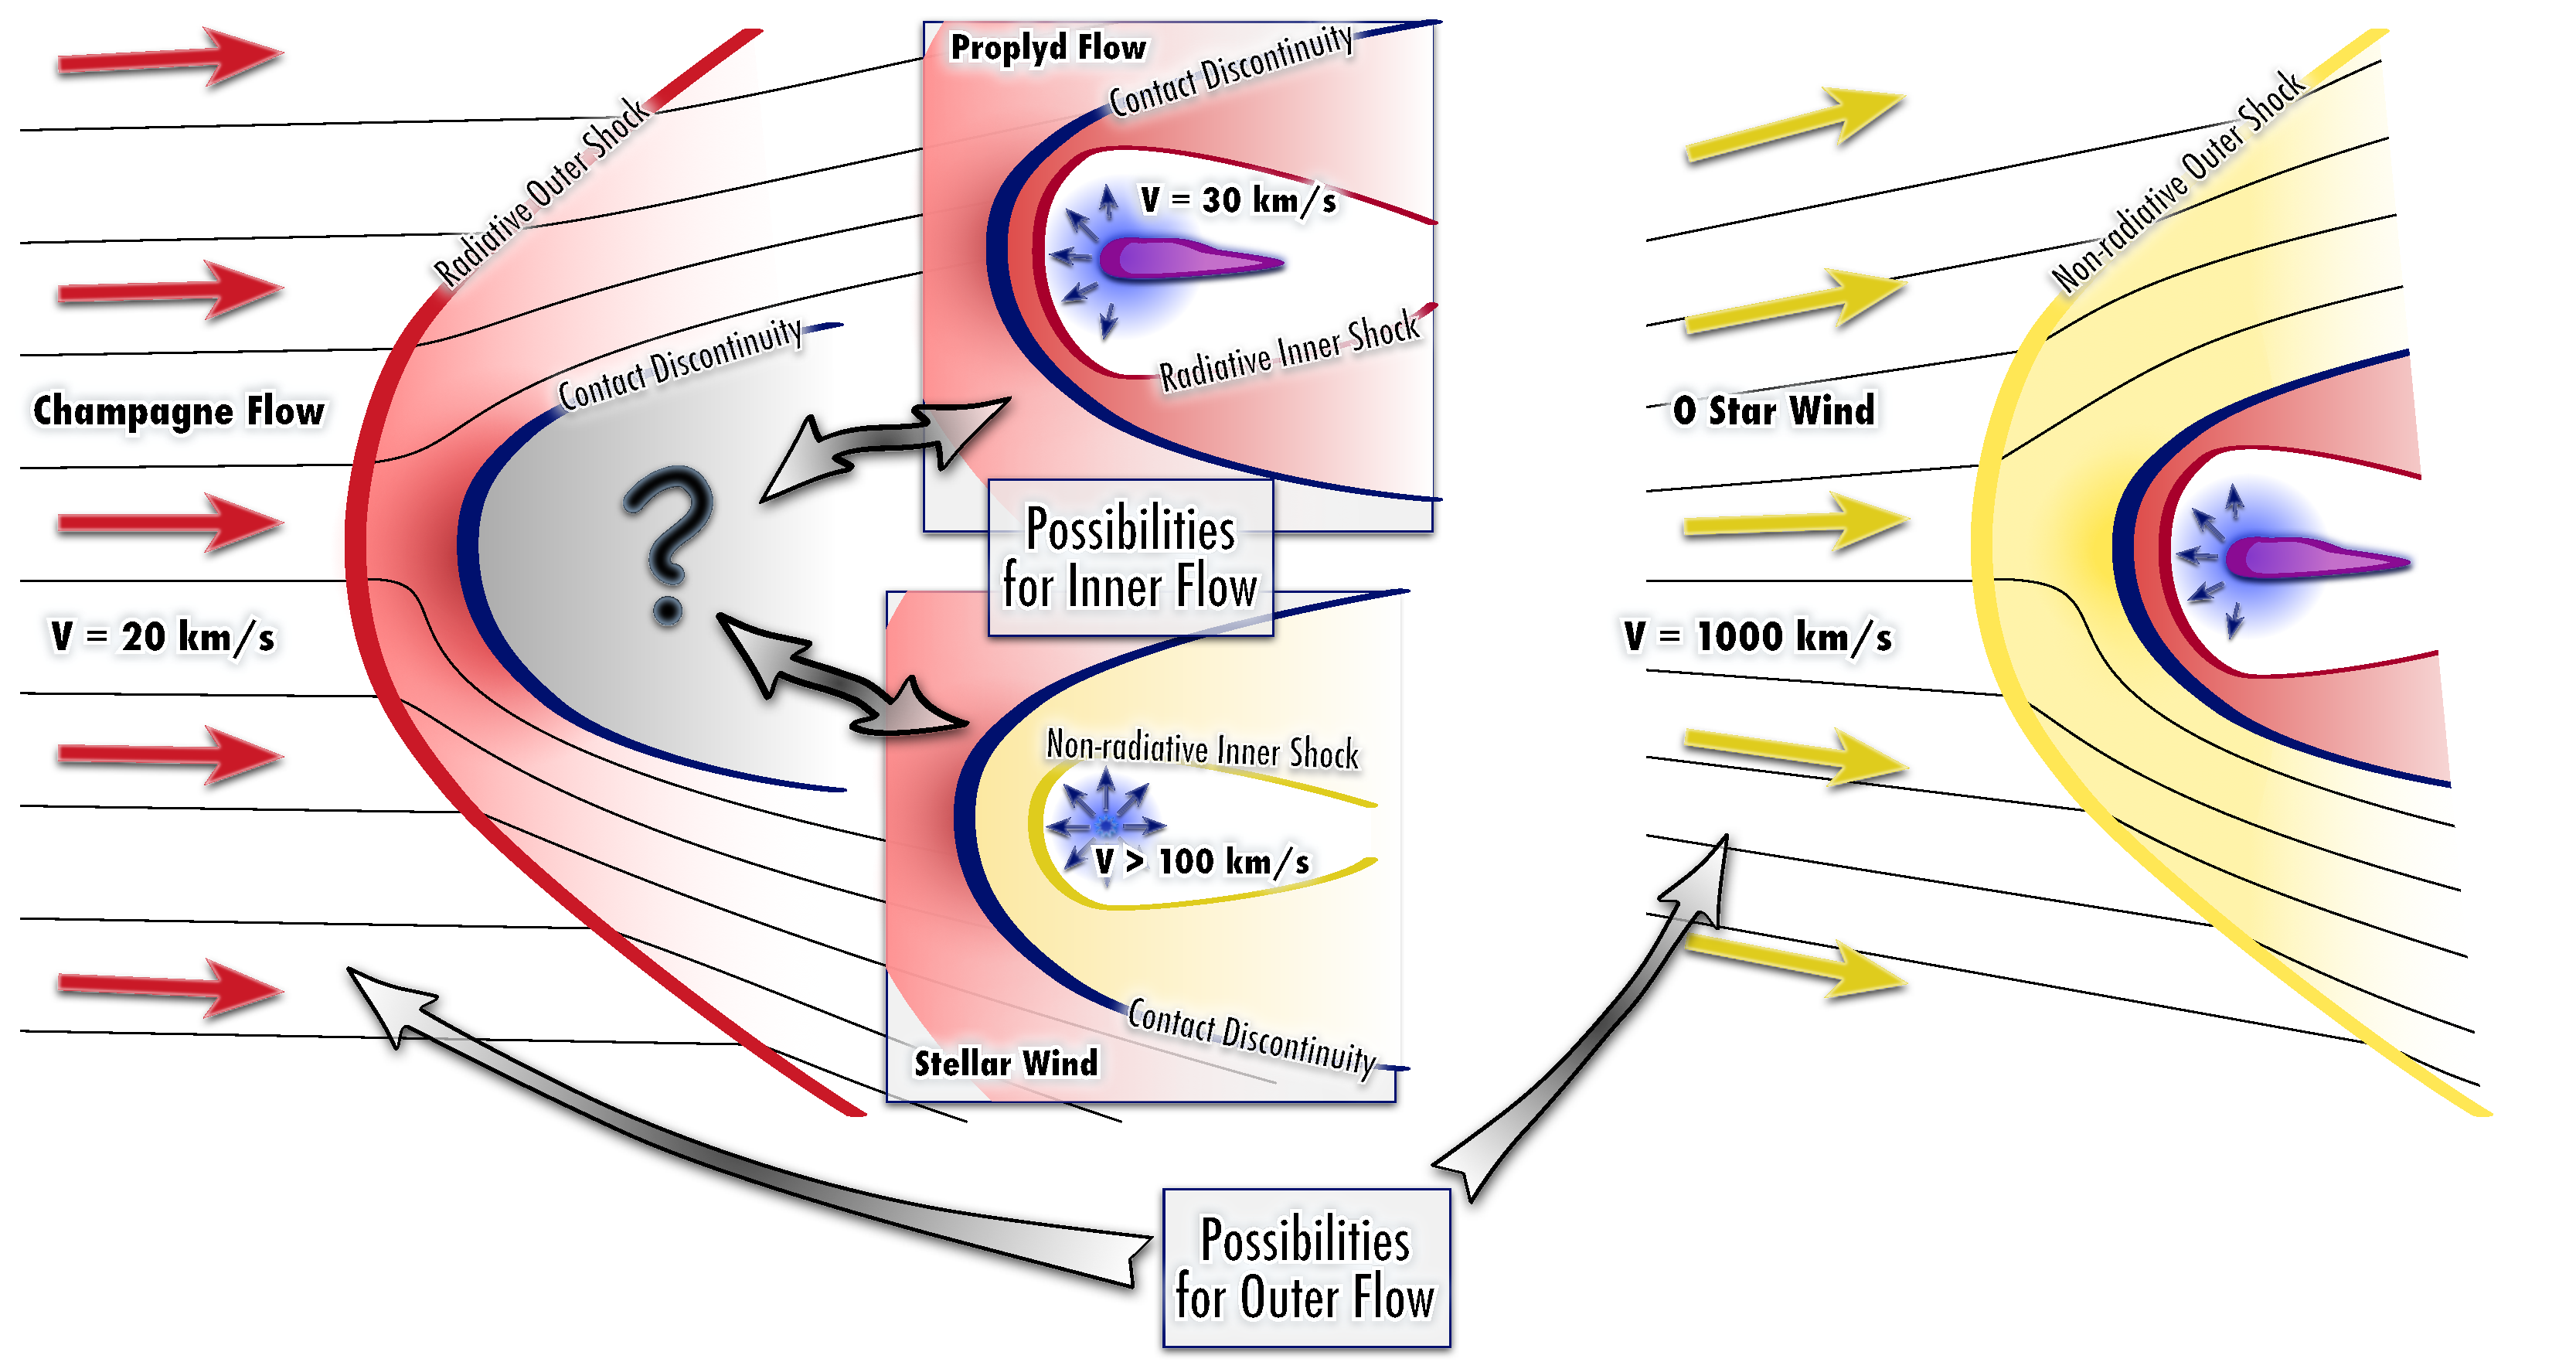
\includegraphics[width=\linewidth]{./Figures/LL-outer-inner-extend-Luis}
  \caption[Posibles escenarios para los flujos en interacción de los choques de proa en ON]{Posibles escenarios para los flujos en interacción de los choques de proa en ON. Izquierda: Un flujo de champaña transónico interactúa ya sea con el flujo fotoevaporado de un proplyd o con un viento estelar, este caso aplica para los arcos más alejados de \thC{}. Derecha: El viento estelar proveniente de una estrella tipo O interactúa con el flujo fotoevaporado de un proplyd. Aplica para los proplyds más cercanos a \thC{}.}
  \label{fig:LL-scheme}
\end{figure}

\begin{figure}
  \centering
  \includegraphics[width=\linewidth]{./Figures/radius-methodology-Luis}
  \caption[Metodología para la medición de la forma del choque de proa]{Metodología para la medición de la forma del choque de proa. Para un arco dado, se traza la posición de las dos cáscaras utilizando marcas con el programa DS9 para imágenes astronómicas (las cruces en la figura). Posteriormente, con un ajuste de mínimos cuadrados se ajusta un círculo a las marcas de cada cáscara para obtener el radio de curvatura aparente $R_c$ (línea roja rayada). El radio en el ápex $R_0$ se obtiene como la distancia mínima entre la posición de la estrella y el ajuste circular y por último el grosor $H$ se obtiene como la diferencia entre ambas mediciones de $R_0$, suponiendo que estén disponibles. PA es el ángulo de orientación de la línea que conecta la estrella central con el centro de curvatura del choque, medido a parir del norte en sentido contrario a las manecillas del reloj (hacia el este). La definición de $R_0$ y $R_c$ es tratada a más profundidad en \S \ref{sec:char-rad}.}
  \label{fig:methodology-LL}
\end{figure}

\begin{figure}
  \centering
%  \begin{tabular}{cc}
    \includegraphics[width=\linewidth]{./Figures/LL1-Bally_01-images}\\  \includegraphics[width=\linewidth]{./Figures/LL4-Bally_24-images}\\ % \includegraphics[width=0.9\linewidth]{./Figures/LL5-Bally_07-images}  
%  \end{tabular}
  \caption[Ejemplos de objetos LL obtenidos del catálogo de \citet{Gutierrez-Soto:2015a}]{Ejemplos de objetos LL obtenidos del catálogo de \citet{Gutierrez-Soto:2015a}. A la derecha de cada panel se observa el objeto con las mediciones superpuestas de los radios característicos $(R'_0, R'_c)$ para las cáscaras exterior e interior o solo para una dependiendo del objeto. La escala de grises muestra el brillo, la barra amarilla indica la escala del objeto y las etiquetas mestran el nombre del objeto, el instrumento que se utilizó para obtener la imagen y la fecha en que se obtuvo.}
  \label{fig:Luis-mosaic-1}
\end{figure}

\begin{figure}
  \centering
  \ContinuedFloat
  \captionsetup{list=off, format=cont}
  \includegraphics[width=\linewidth]{./Figures/LL6-Bally_08-images} \includegraphics[width=\linewidth]{./Figures/042-628-Bally_16-images}  %\includegraphics[width=0.9\linewidth]{./Figures/109-246-Bally_01-images}
  \caption{}
  \label{fig:Luis-mosaic-2}
\end{figure}


\begin{figure}
  \centering
%  \begin{tabular}{cc}
    \includegraphics[width=\linewidth]{./Figures/ll-pos-image-Luis}
%  \end{tabular}
  \caption[Mapa de objetos del catálogo de \citet{Gutierrez-Soto:2015a} dentro de ON]{Mapa de objetos del catálogo de \citet{Gutierrez-Soto:2015a} dentro de ON. Las flechas de colores contienen la línea que une la posición del objeto central con el eje de curvatura de cada cáscara. Los puntos rojos representan objetos que no tienen un choque de proa visible. En el recuadro blanco se muestra el ID de cada objeto, siguiendo la nomenclatura de \citet{ODell:1994a}. La zona marcada con el cuadrado amarillo se encuentra amplificada en la continuación de esta figura.}
  \label{fig:orion-map-LL}
\end{figure}

\begin{figure}
  \centering
  \ContinuedFloat
  \captionsetup{list=off, format=cont}  
  \includegraphics[width=\linewidth]{./Figures/ll-pos-image-zoom-Luis}
  \caption{}
  \label{orion-map-LL-2}
\end{figure}


\section{Estrellas ``Errantes''}
\label{sec:runaway}

Otro tipo de choques de proa estelares ocurren cuando los vientos de estrellas \textit{errantes} (runaway stars), usualmente de tipos espectrales OB, con velocidades mayores a \SI{30}{km.s^{-1}} interactúan con el medio interestelar \citep{Kobulnicky:2016}. Estas estrellas adquieren estas velocidades cuando sufren encuentros dinámicos cercanos dentro del cúmulo donde se formaron o bien cuando forman parte de un sistema binario cerrado y uno de los miembros explota como supernova.

En la figura \ref{fig:runaway} se muestran algunos ejemplos típicos de choques de proa producidos por estrellas errantes. Los colores en cada imagen representan a la banda de \SI{24}{\mu.m} del Telescopio Espacial Spitzer, o bien la de \SI{22}{\mu.m} del catálogo WISE para el color rojo, para el color verde puede ser la banda de \SI{8}{\mu.m} de Spitzer o la de \SI{12}{\mu.m} de WISE, y al color azul le corresponde la banda de \SI{4.5}{\mu.m} de Spitzer o WISE y los objetos mostrados son, de arriba a abajo y de izquierda a derecha: $\zeta$\,Oph, AE Aur, HD136003, HD150898, HD155755 y HD143275, y por último, la flecha blanca indica la magnitud y dirección del movimiento propio de la estrella.

\begin{figure}
  \centering
  \includegraphics[width=0.7\linewidth]{./Figures/kobulnicky}
  \caption[Ejemplos de choques de proa en infrarrojo producidos por estrellas errantes]{Ejemplos de choques de proa en infrarrojo producidos por estrellas errantes, tomados por el telescopio espacial Spitzer o del catálogo WISE. Los colores representan las bandas de \SI{24}{\mu.m} de Spitzer o \SI{22}{\mu.m} de WISE (rojo), \SI{8}{\mu.m} de Spitzer o \SI{12}{\mu.m} de WISE (verde) y \SI{4.5}{\mu.m} de de Spitzer o WISE (azul). Los objetos mostrados son: $\zeta$\, Oph (G006.2812+23.5877; arriba izquierda), AE Aur (G172.0813-02.2592; arriba derecha), HD136003 (G322.6802+00.9060; centro izquierda), HD150898 (G329.9790-08.4736; centro derecha), HD155755 (G348.7967+00.1455; abajo izquierda) y HD143275 (G350.0969+22.4904; abajo derecha). La magnitud y dirección del movimiento propio se muestra con las flechas blancas \citep{Kobulnicky:2016}.}
  \label{fig:runaway}
\end{figure}

\section{Estrellas AGB y Supergigantes Rojas}
\label{sec:AGBs}
Otro tipo de choques de proa estelares se forma cuando estrellas en sus fases evolutivas finales, tales como estrellas AGB y supergigantes rojas pierden material a través de fuertes vientos ($\sim 10^{-9}$ -- \SI{e-4}{M_\odot.yr^{-1}}, \citet{Prialnik}) que producen choques al interaccionar con el Medio Interestelar \citep{Cox:2012}.

En la figura  \ref{fig:fermata} se muestran ejemplos de estrellas AGB y supergigantes en infrarrojo lejano que forman parte del programa MESS (Mass-loss of Evolved StarS, \citet{Groenewegen:2011}) que utilizan el instrumento PACS (Photodetector Array Camera Spectrometer), donde se usan los filtros de \SI{70}{\mu.m} y \SI{160}{\mu.m}, y que muestran choques tipo ``fermata''. Otras formas que se observan son tipo ``ojos'', ``anillos'' e ``irregulares'' (ver tabla \ref{tab:morphology-AGB}).

\begin{figure}
  \centering
  \includegraphics[width=0.5\linewidth]{./Figures/Cox-fermata}
  \caption[Interacciones tipo ``fermata'' de los objetos R\,Scl, NML\,Tau, W\,Ori, W\,Pic y $\alpha$\,Ori]{Interacciones tipo ``fermata'' de los objetos R\,Scl, NML\,Tau, W\,Ori, W\,Pic y $\alpha$\,Ori tomadas con PACS en los filtros de \SI{70}{\mu.m} (izquierda) y \SI{160}{\mu.m} (derecha). La barra blanca mide 1' en la imagen, así como su respectivo tamaño físico. En todos los páneles el norte se ubica hacia arriba y el este a la izquierda. La línea negra indica la velocidad y dirección de la velocidad espacial de la estrella, adoptando una escala tal que \SI{1}{km.s} corresponde a 1'' en la imagen \citep{Cox:2012}. Nota adicional. R\,Scl tiene una cáscara esférica interna no visible en la imagen.}
  \label{fig:fermata}
\end{figure}

\begin{table}
  \centering
  \begin{tabular}{llc}
    \toprule
    Clase & Descripción & Forma \\
    \midrule
    I & Fermata & \includegraphics[scale=0.03]{./Figures/fermata} \\
    II & Ojos   & \includegraphics[scale=0.03]{./Figures/eyes} \\
    III & Anillos & \includegraphics[scale=0.02]{./Figures/ring} \\
    IV & Irregulares & \\
    \bottomrule
  \end{tabular}
  \caption{Clasificación morfológica de choques de proa estelares de estrellas AGB y supergigantes \citep{Cox:2012}.}
  \label{tab:morphology-AGB}
\end{table}


%\includegraphics[width=0.1\linewidth]{./Figures/tux-development}

\chapter{Conceptos fundamentales}
\label{sec:Modelo-generico}
Para este trabajo consideramos en general dos modelos de interacción de vientos:
\begin{itemize}
\item Una fuente localizada en el origen que emite un viento esférico que puede ser isotrópico o anisotrópico (figura \ref{fig:isotropic-aniso}) no acelerado que interactúa con el viento esférico isotrópico de otra fuente que se encuentra a una distancia $D$ de la primera(figura \ref{fig:crw-esquema}). A los choques de proa resultantes se conocen como ``Cantoides'' y ``Ancantoides'', respectivamente.
\item Una fuente localizada en el origen que emite un viento esférico isotrópico no acelerado que interactúa con un viento plano paralelo no acelerado y densidad constante (figura ). Los choques resultantes en este caso se conocen como ``Wilkinoides''.
\end{itemize}
El sitema en su conjunto tiene simetría cilíndrica.
\begin{figure}
  \includegraphics[width=0.5\linewidth]{./Figures/anisotropic-arrows}
  \caption{Representación esquemática de vientos con diferentes anisotropías: Arriba izquierda: Viento isotrópico esférico. Arriba derecha: viento isotrópico hemisférico. Abajo: Vientos anisotrópicos donde el parámetro $k$ indica el grado de anisotropía (ver capítulo \ref{chap:hipersonica})}
    \label{fig:isotropic-aniso}
\end{figure}
\begin{figure}
  \begin{tabular}{lr}
    \includegraphics[width=0.45\linewidth]{./Figures/bowshock-crw-variables} &
    \includegraphics[width=0.45\linewidth]{./Figures/wilkinoid}
  \end{tabular}
  \caption{Izquierda: Representación esquemática del problema de interacción de dos vientos esféricos: Dos fuentes separadas por una distancia $D$ emiten un viento radial que forma un choque de proa a una distancia $R$ del origen. El sistema tiene geometría cilíndrica siendo el eje $z$ el eje de simetría. La forma del choque es función únicamente del ángulo polar $\theta$, medido a partir del origen. Otro ángulo que es de utilidad es $\theta_1$, que corresponde al ángulo polar medido a partir de la posición de la otra fuente. Cuando el viento interior tiene densidad constante y es esférico, denominamos al choque resultante como ``cantoide'', mientras que si su densidad sigue una ley de potencias de $\cos\theta$, siguiendo la ecuación (\ref{eq:anisotropic-density}) del capítulo \ref{chap:hipersonica}, será un choque ``ancantoide''. Derecha: Representación esquemática de la interacción de un choque esférico e isotrópico con una corriente plano--paralela de densidad y velocidad constantes. El choque resultante es en este caso de tipo ``wilkinoide''}
    \label{fig:crw-esquema}
\end{figure}

\section{Planitud y ``Alatud''}
\label{sec:char-rad}
Las cantidades medibles que nos ayudan a caracterizar un choque de proa las llamamos ``Radios característicos'' (ilustrados en la figura \ref{fig:char-radii}):
\begin{itemize}
\item Radio del choque en la dirección del eje del ápex. Denotado como $R_0$
\item Radio en dirección perpendicular al ápex. Denotado como $R_{90}$
\item Radio de curvatura en el ápex. Denotado como $R_c$. En el apéndice \ref{app:math-curvature-radius} se muestra el procedimiento para obtener este radio para una curva genérica continua y derivable.
\end{itemize}

\begin{figure}
  \includegraphics[width=0.5\linewidth]{./Figures/characteristic-radii}
  \caption{Representación esquemática de los radios característicos de un choque de proa}
  \label{fig:char-radii}
\end{figure}
Un último parámetro es el ángulo asintótico de apertura de las alas, denotado como $\theta_\infty$. Sin embargo, esta medida solo aplica para choques cuyas alas son asintóticamente cónicas, y aún para éstos en la mayoría de los casos es dificil de medirlo debido a que el ángulo polar $\theta$ tiende al valor asintótico muy lentamente y además la emisión de las alas es bastante débil. Por otro lado, los radios característicos $(R_0, R_c, R_{90})$ son medibles observacionalmente en la mayoría de los casos. A partir de éstos, podemos determinar dos parámetros adimensionales llamados ``planitud'' y ``alatud''. El primero de éstos es una medida de qué tan plano es el choque de proa en la nariz o ``apex'', y lo denotamos con la letra griega $\Pi$, mientras que el segundo es una medida de qué tanto se abren las alas del choque de proa, y lo denotamos con la letra griega $\Lambda$. Ambos parámetros se definen a continuación:

\begin{align}
  \Pi \equiv \frac{R_c}{R_0} \label{eq:planitude}\\
  \Lambda \equiv \frac{R_{90}}{R_0} \label{eq:alatude}
\end{align}

\section{Cuádricas de Revolución}
\label{sec:quadrics}
\newcommand\Sin{\ensuremath{\mathcal{S}}}
\newcommand\Cos{\ensuremath{\mathcal{C}}}
\newcommand\Cot{\ensuremath{\mathcal{T}}}
\newcommand\Q{\ensuremath{\mathcal{Q}}}
\newcommand\fQi{\ensuremath{f_{\scriptscriptstyle \Q, i}}}
En el caso general es difícil encontrar la forma aparente para un choque de proa siguiendo el formalismo desarrollado en la sección anterior, por lo que optamos por aproximar la forma éstos con una de las superficies más simples: las \textit{cuádricas de revolución}, que son superficies de revolución de las curvas cónicas. Dado el modelo general descrito en la \S \ref{sec:Modelo-generico}, haremos algunas restricciones para las superficies cuádricas que utilizaremos en este trabajo:
\begin{itemize}
  \item El eje focal se encuentra alineado con el eje $x$
  \item La posición del foco de la superficie cuádrica no necesariamente coincide con la posición de la fuente
  \item En el caso de las hipérbolas, solo tomamos una de las ramas de ésta.
\end{itemize}
Implementando dichas restricciones, utilizamos la representación paramétrica de las curvas cónicas en términos de un parámetro adimensional denotado con la letra $t$:
\begin{align}
  x &= x_0 + \sigma a\Cos(t) \\
  y &= b\Sin(t) 
\end{align}
Donde:
\begin{align}
  \Cos(t), \Sin(t) &=\left\lbrace
  \begin{array}{lr}
    \cos{t}, \sin t & \mathrm{elipses}\\
    \cosh{t}, \sinh{t} & \mathrm{hipérbolas}       
  \end{array}\right. \\
  \sigma &= \left\lbrace
  \begin{array}{lr}
    +1 & \mathrm{elipses} \\
    -1 & \mathrm{hipérbolas}
  \end{array}\right. \\
  x_0 &= R_0 -\sigma a \label{eq:x0} 
\end{align}
Donde $a$ y $b$ representan la longitud de los semi-ejes de la cónica en cuestión (Figura \ref{fig:conics}). $x_0$ representa la distancia entre el centro de la cónica y el origen. 

La forma polar del choque de proa $R(\theta)$ viene dada por:

\begin{align}
  \tan\theta &= \frac{b\Sin(t)}{a\Cos(t) + x_0} \label{eq:t-th-conversion} \\
  R &= \left(\left(a\Cos(t) + x_0\right)^2 + b^2\Sin^2(t)\right)^{1/2} 
\end{align}
El tipo de cónica lo podemos caracterizar mediante el parámetro $\Q$, donde:
\begin{align}
  \Q \equiv \sigma\frac{b^2}{a^2} \label{eq:conic-parameter-a-b}
\end{align}
Para las superficies abiertas (hiperboloides) tenemos que $\Q < 0$, mientras que para las superficies cerradas tenemos que $\Q > 0$. Casos particulares son la esfera $\Q = 1$ y el paraboloide $\Q = 0$. De manera equivalente se puede definir el ángulo $\theta_Q$ como sigue:
\begin{align}
  \tan\theta_Q = \sigma \frac{b}{a} \label{eq:thc}
\end{align}
Este ángulo se relaciona con la excentricidad de las cónicas (y que sustituye a esta última en este trabajo) como se muestra a continuación:
\begin{align}
  \tan\theta_Q = \sigma\sqrt{\left|1-e^2\right|}
\end{align}
\begin{figure}
  \begin{tabular}{cc}
    \includegraphics[width=0.4\linewidth]{./Figures/ellipse_edited} &
    \includegraphics[width=0.5\linewidth]{./Figures/hyperbola_edited}
  \end{tabular}
  \caption{Representación esquemática de: Izquierda: Elipse. Y, derecha: Hipérbola. En ambos casos se ilustran los parámetros relevantes de éstas y los radios característicos}
  \label{fig:conics}
\end{figure}

\begin{figure}
  \includegraphics[width = 0.5\linewidth]{./Figures/conic1}
  \caption{Familia de curvas cónicas, donde el valor del parámetro $\theta_Q$ varía desde $\theta_Q < 0$ (hipérbolas) hasta $\theta_Q > 0$ (elipses). Casos especiales son $\theta_Q = 0$ (parábola) y $\theta_Q = 45^\circ$ (círculo). Este parámetro sustituye en este trabajo a la excentricidad.}
  \label{fig:conics-family}
\end{figure}
El set de parámetros $(a, x_0, \Q)$ es suficiente para caracterizar a nuestras cuádricas de revolución: $\Q$ nos indica el tipo de cónica, $a$ establece la escala y $x_0$ el desplazamiento del centro a lo largo del eje x. Sin embargo, para futuras aplicaciones tanto a modelos de interacción de vientos como a observaciones (capítulos \ref{chap:hipersonica} y \ref{chap:proplyds}) nos sería util hacer la caracterización mediante los parámetros $(R_0, \Pi, \Lambda)$ (ver \S \ref{sec:char-rad}). Las equivalencias entre los dos sets de parámetros los calculamos a continuación:
\begin{align} 
  R_c &= \frac{b^2}{a} = a|\Q|\label{eq:R-curv-conic}\\
  R^2_{90} &= b^2\sigma\left(1 - \frac{x^2_0}{a^2}\right) = \Q\left(a^2 - x^2_0\right)\label{eq:R90-conic} 
\end{align}
Combinando las ecuaciones (\ref{eq:planitude}, \ref{eq:alatude}, \ref{eq:x0}, \ref{eq:conic-parameter-a-b}, \ref{eq:R-curv-conic}, \ref{eq:R90-conic}), obtenemos lo siguiente:

\begin{align}
  R_0 &= x_0 + \sigma a \label{eq:R0}\\
  \Pi &= \frac{a|\Q|}{x_0 + \sigma a} = \frac{a\Q}{\sigma\left(x_0 + \sigma a\right)} = \frac{a\Q}{\left(a + \sigma x_0\right)}\label{eq:quadric-planitude}\\
  \Lambda &= \left(\Q\frac{a-\sigma x_0}{a + \sigma x_0}\right)^{1/2}
\end{align}

De aquí podemos escribir el parámetro de las cuádricas $\Q$ en términos de la planitud y la alatud:

\begin{align}
  \Q = 2\Pi - \Lambda^2 \label{eq:quadric-parameter-pi-lambda}
\end{align}

Por tanto, el signo de $2\Pi - \lambda^2$ determina si una cuádrica es esferoidal o hiperboloidal. En la figura \ref{fig:conics-family} mostramos como, para planitud constante, podemos tener una familia de cónicas variando únicamente la alatud, y por consiguiente, el parámetro $\Q$.

\section{Proyección en el Plano del Cielo}
\label{sec:projection}

Para un choque de proa que es la vez geométricamente delgado y ópticamente delgado, únicamente se observa el borde de éste por
abrillantamiento al limbo, por lo tanto, su orientación respecto a la línea de visión modifica su forma respecto a la forma real del
choque. Para ello, rotamos el sistema de referencia del choque de proa en coordenadas cartesianas, denotado por $(x, y, z)$, por un ángulo que llamamos \textit{inclinación}, denotado por $i$, en el plano $xz$, de modo que la transformación entre el sistema de refencia del choque y el sistema de referencia del plano del cielo, denotado por
$(x', y', z')$ queda como sigue:
\begin{align}
  \left(
  \begin{array}{c}
    x' \\ y' \\ z'
  \end{array}
  \right) &=
  \left(
  \begin{array}{c}
    x\cos i - z\sin i \\ y' \\ z\cos i + x\sin i
  \end{array}
  \right)
  \label{eq:rotation}
\end{align}
Por otro lado, la forma tridimensional del choque de proa viene dado por:
\begin{align}
  \left(
  \begin{array}{c}
    x \\ y \\ z
  \end{array}
  \right) &=
            R(\theta)\left(
            \begin{array}{c}
              \cos\theta \\
              \sin\theta\cos\phi \\
              \sin\theta\sin\phi
            \end{array}
            \right)
\end{align}
La relación entre ambos sistemas de referencia se ilustra en la figura \ref{fig:reference}.
\begin{figure}
  \includegraphics[width=0.5\linewidth]{./Figures/projection-pos}
  \label{fig:reference}
  \caption{Sistema de referencia del choque vs sistema de referencia del plano del cielo. Los ejes $x'$ y $y'$ se encuentran en el plano del cielo, mientras el eje $z'$ es paralelo a la línea de visión. Solo la región del choque cuya tangente sea paralela a la línea de visión será visible por abrillantamiento al limbo.}
\end{figure}

\subsection{Vectores normal y tangente a la superficie}

Si definimos los vectores $\hat{n}$ y $\hat{t}$, como los vectores normal y tangente a la superficie, respectivamente para $\phi$ constante. En el caso $\phi = 0$ (figura \ref{fig:unit-vec}), ambos vectores se encuentran en el plano $xy$ y es fácil mostrar que:
\begin{align}
  \hat{t}_0 =
  \left(
  \begin{array}{c}
    -\cos\alpha \\
    \sin\alpha \\
    0
  \end{array}
  \right)
  \quad \mathrm{y} \quad
  \hat{n}_0 =
  \left(
  \begin{array}{c}
    \sin\alpha \\
    \cos\alpha \\
    0
  \end{array}
  \right)
  \label{eq:unit-vec}
\end{align}
Donde:
\begin{align}
  \tan\alpha = -\frac{dy}{dx} = \frac{1+\omega\tan\theta}{\tan\theta-\omega}
\end{align}
y:
\begin{align}
  \omega(\theta) = -\frac{1}{R}\frac{dR}{d\theta} 
\end{align}
Para otros valores de $\phi$, basta con hacer una rotación de las ecuaciones (\ref{eq:unit-vec}) alrededor del eje $x$. Para la conversión al sistema de referencia del plano del cielo se utiliza la ecuación (\ref{eq:rotation}):
\begin{align}
\begin{split}
  \hat{n}' &= \frac{1}{\left(1 + \omega^2\right)^{1/2}} \\
           & \times \left(
             \begin{array}{c}
               (\cos\theta+\omega\sin\theta)\cos i-(\sin\theta-\omega\cos\theta)\sin i\sin\phi\\
               (\sin\theta-\omega\cos\theta)\cos\phi \\
               (\cos\theta+\omega\sin\theta)\sin i+(\sin\theta-\omega\cos\theta)\sin\phi\cos i
             \end{array}
                    \right) \\
\end{split}\\
\begin{split}
    \hat{t}' &= \frac{1}{\left(1 + \omega^2\right)^{1/2}} \\
           & \times \left(
             \begin{array}{c}
               -(\sin\theta-\omega\cos\theta)\cos i-(\cos\theta+\omega\sin\theta)\sin i\sin\phi\\
               (\cos\theta+\omega\sin\theta)\cos\phi \\
               -(\cos\theta+\omega\sin\theta)\sin i+(\sin\theta-\omega\cos\theta)\sin\phi\cos i
             \end{array}
             \right)
\end{split} 
\end{align}


\begin{figure}
  \includegraphics[width=0.6\linewidth]{./Figures/bowshock-unit-vectors}
  \caption{Vectores unitarios normal y tangente a la superficie $R(\theta)$
    en un plano de azimuth $\phi$ constante.}
    \label{fig:unit-vec}
\end{figure}

\subsection{Línea tangente}
\label{sec:tangent-line}
Debido a que el choque es ópticamente delgado y geométricamente delgado, solo la región del choque cuya tangente sea paralela a la
línea de visión seré visible. Esto corresponde a una curva que denominamos \textit{línea tangente}, que debe cumplir con la siguiente
condición:
\begin{align}
  \hat{n}'\boldsymbol{\cdot} \hat{z}' = 0
\end{align}
Denotamos como $\phi_T$ al ángulo azimutal que cumple la condición anterior para una inclinación dada, en función del ángulo polar $\theta$:
\begin{align}
  \sin\phi_T = \tan i\tan\alpha = \tan i\frac{1+\omega\tan\theta}{\omega-\tan\theta}
  \label{eq:phi-tan}
\end{align}
De esta manera, la forma de la línea tangente del choque de proa, a la que llamamos \textit{forma proyectada} viene dada por:
\begin{align}
  \left(
  \begin{array}{c}
    x'_T \\
    y'_T \\
    z'_T
  \end{array}
  \right) =
  R(\theta)\left(
  \begin{array}{c}
    \cos\theta\cos i - \sin\theta\sin\phi_t\sin i \\
    \sin\theta\left(1-\sin^2\phi_T\right)^{1/2} \\
    \cos\theta\sin i + \sin\theta\sin\phi_T\cos i
  \end{array}
  \right) \label{eq:proj-shape}
\end{align}
En el caso general, $z'_T$ no es una función lineal de $x'_T$ y $y'_T$, por lo que la línea tangente no se encuentra en un plano. La forma aparente $(x'_T, y'_T)$  de la línea tangente también puede escribirse en coordenadas polares $(R', \theta')$, donde:
\begin{align}
  R'(\theta) = \left(x'^2_T + y'^2_T\right)^{1/2} & \mathrm{y} & \tan\theta' = \frac{y'_T}{x'_T}
  \label{eq:polar}
\end{align}
Es de notar a su vez que la ecuación (\ref{eq:phi-tan}) no tiene solución para valores arbitrarios de $\theta$ y de la inclinación, puesto que se requiere que $\left|\sin\phi_T\right| < 1$. Por tanto, la línea tangente solo existe para valores de $\theta$ tales que $\theta < \theta_0$ donde $\theta_0$ es el valor de $\theta$ en el eje de simetría de la línea tangente proyectada $(\theta'(\theta_0) = 0)$ y que se obtiene resolviendo la siguiente ecuación implícita:
\begin{align}
  \tan\theta_0 = \frac{|\tan i| + \omega(\theta_0)}{1 - \omega(\theta_0)|\tan i|}
  \label{eq:th-0}
\end{align}
Esto implica que si el choque de proa es suficientemente ``abierto'' $(\alpha > \alpha_{min})$, entonces para inclinaciones tales que
$|i| > 90^\circ - \alpha_{min}$ no existirá la línea tangente para ningún valor de $\theta$, es decir, el choque de proa se encontrará sufientemente ``de cara'' como para que ya no parezca un choque de proa para el observador.

\subsection{Planiud y Alatud proyectadas: caso general}

En orden de comparar la forma $R(\theta)$ con observaciones, es útil definir los radios característicos $R'_0$ y $R'_{90}$, donde $R'_0$ es el radio del eje de simetría aparente y $R'_{90}$ es el radio aparente en la dirección perpendicular a $R'_0$. Es decir
$R'_0 = x'_T(y'_t=0)$ y $R'_{90} = y'_t(x'_t = 0)$. Utilizando las ecuaciones (\ref{eq:phi-tan}) y (\ref{eq:proj-shape}) encontramos que:
\begin{align}
R'_0 = R(\theta_0)\cos(\theta_0 + i)
\label{eq:R0p}
\end{align}
Donde $\theta_0$ es la solución de la ecuación (\ref{eq:th-0}), y
\begin{align}
  R'_{90} = R(\theta_{90})\sin\theta_{90}\left(1-\sin^2\phi_T(\theta_{90})\right)^{1/2}
  \label{eq:R90p}
\end{align}
donde $\theta_{90}$ es la solución de la siguiente ecuación implícita:
\begin{align}
  \cot\theta_{90} = \frac{1 - \left(1+\omega(\theta_{90})^2\sin^22i\right)^{1/2}}
  {2\omega(\theta_{90})\cos^2i}
  \label{eq:th90}
\end{align}

\subsection{Aplicación a las Cuádricas de Revolución}

El objetivo de esta sección es obtener la forma proyectada de las cuádricas de revolución, puesto que son una aproximación buena y mucho más sencilla a la forma real de un choque de proa. Para esto es conveniente utilizar un sistema de referencia donde el origen se ubica en el centro de la sección cónica:

\begin{align}
  (X, Y, Z) = (x-x_0, y, z)
\end{align}

De esta manera, la forma de la cuádrica de revolución es:

\begin{align}
  X &= a\Cos(t) \\
  Y &= b\Sin(t)\cos\phi \\
  Z &= b\Sin(t)\sin\phi
\end{align}

Siguiendo el procedimiento mostrado en la \S \ref{sec:projection} calculamos el ángulo azimutal $\phi$ que cumple con el criterio de ser tangente a la línea de visión: 

\begin{align}
  \sin\phi_T = \frac{b\Cos(t)}{a\Sin(t)}\tan i 
\end{align}
Ahora utilizamos la ecuación (\ref{eq:rotation}) para obtener la forma aparente de una cuádrica dada:
\begin{align}
  X'_T &= \frac{\Cos(t)}{a\cos i}\left(a^2\cos^2 i + \sigma b^2\sin^2 i\right)
  \label{eq:x-prime-proj}\\
  Y'_T &= b\Sin(t)\left(1 - \frac{b^2\Cos^2(t)}{a^2\Sin^2(t)}\tan^2 i\right)^{1/2}
  \label{eq:y-prime-proj}
\end{align}
Podemos mostrar que la forma proyectada de una sección cónica (elipse o hipérbola), es de la misma clase que la sección cónica original. Si ese fuera el caso, entonces podemos escribir las ecuaciones (\ref{eq:x-prime-proj}, \ref{eq:y-prime-proj}) de la siguiente manera:
\begin{align}
  X'_T &= a'\Cos(t') \label{eq:xtprime}\\
  Y'_T &= b'\Sin(t') \label{eq:ytprime}
\end{align}

Después de un poco de álgebra encontramos que nuestra suposición es consistente, con las siguientes equivalencias:

\begin{align}
  a' &= a\cos i \fQi \label{eq:a-prime}\\
  b' &= b \label{eq:b-prime}\\
  \Cos(t') &= \fQi \Cos(t)
\end{align}

Donde introducimos el factor de proyección de las cuádricas:
\begin{align}
  \fQi = \left(1 + \Q\tan^2i\right)^{1/2}
\end{align}


%Dos cantidades que nos van a ser de utilidad son los valores del parámetro $t$ que denominaremos $t_0$ y $t_{90}$ y son tales que $t'(t_0) = 0$ y $t'(t_{90}) = \frac{\pi}{2}$ o bien $y'_T(t_0) = 0$ y $x'_T(t_{90}) = 0$. De esta manera obtenemos las siguientes ecuaciones implícitas evaluando las ecuaciones (\ref{eq:x-prime-proj}) y(\ref{eq:y-prime-proj}) en $t=t_{90}$ y $t=t_0$ respectivamente:
%\begin{align}
%  \Cot(t_0) &= \frac{a}{b}\cot{i} = \frac{\cot{i}}{\left|\tan\theta_c\right|} %\label{eq:t0}\\
%  \Cos(t_{90}) &= -\frac{ax_0\cos^2{i}}{a^2\cos^2{i}\pm b^2\sin^2{i}} \label{eq:t90}
%\end{align}
Como ya demostramos que la forma proyectada de la línea tangente de una superficie cúadrica es una sección cónica del mismo tipo, entonces podemos determinar la forma proyectada reutilizando las ecuaciones (\ref{eq:R0}-\ref{eq:quadric-parameter-pi-lambda}) sustituyendo las cantidades no primadas por sus equivalentes primados. De esta manera, utilizando las ecuaciones (\ref{eq:conic-parameter-a-b}, \ref{eq:a-prime}, \ref{eq:b-prime}) encontramos que el parámetro de las cuádricas para la forma proyectada es:

\begin{align}
  \Q' = \frac{\Q}{\fQi^2 \cos^2 i}\label{eq:Q-prime}
\end{align}

Ahora regresamos al sistema de referencia centrado en la estrella:

\begin{align}
  (x'_T, y'_T) = (X'_T + x'_0, Y'_T)
\end{align}

donde el desplazamiento proyectado $x'_0$ es:

\begin{align}
  x'_0 = x_0\cos i
\end{align}
La proyección de la distancia al ápex viene dada por la versión primada de la ecuación (\ref{eq:R0}):
\begin{align}
  R'_0 &=  x'_0 + \sigma a'\\
  \implies \frac{R'_0}{R_0} &= \cos i\left[1 + \frac{\Pi}{\Q}\left(1 - \fQi\right)\right]
\end{align}

Asimismo la planitud y la alatud proyectada pueden calcularse a partir de las ecuaciones (\ref{eq:quadric-planitude}, \ref{eq:quadric-parameter-pi-lambda}, \ref{eq:a-prime}, \ref{eq:Q-prime}):

\begin{align}
  \Pi' &= \frac{\Pi}{\left(R'_0/R_0\right)\fQi\cos i}\\
  \Lambda' &= \left(2\Pi' - \Q'\right)^{1/2}
\end{align}

%Utilizando las ecuaciones (\ref{eq:x0}), (\ref{eq:a-prime}) y (\ref{eq:b-prime}), utlizando la definición $D' = D\cos i$ e introduciendo la función $f(i;\theta_c)\equiv \left(1 \pm \tan^2\theta_c\tan^2i\right)^{1/2}$ obtenemos ecuaciones explícitas para los radios característicos en el sistema de referencia del plano del cielo en términos de la inclinación:
%\begin{align}
%  \frac{q'}{q} &= 1 \pm \tilde{R}_c\cot^2\theta_c\left(f(i;\theta_c) - 1\right) \\
%  \tilde{R}'_c &= \frac{\tilde{R_c}}{\cos^2if(i;\theta_c)\frac{q'}{q}} \label{eq:Rpc-quad}\\
%  \tan\theta'_c &= \frac{\tan\theta_c}{\cos if(i;\theta_c)} \label{eq:thcp-quad}\\
%  \tilde{R}'_{90} &= \left(\frac{2\tilde{R}_cf(i;\theta_c) \mp
%                    \tan^2\theta_c\frac{q'}{q}}{q'/q}\right)^{1/2}\frac{\sec %i}{f(i;\theta_c)}
%  \label{eq:Rp90-quad}
%\end{align}
%Cuando $\tilde{R}'_{90}$ es medible, entonces es posible hacer diagramas de diagnóstico como
%el de la figura \ref{fig:diagnostic} para comparar con observaciones, independientemente de cualquier modelo de choques de proa.
%\begin{figure}
%  \includegraphics[width=0.5\linewidth]{./Figures/projected-R90-vs-Rc}
%  \caption{Diagrama de diagnóstico $\tilde{R}'_{90}$ vs $\tilde{R}'_c$ para las cuádricas de revolución. En la región sin sombrear se representan las superficies abiertas (hiperboloides, $\theta_c <0$), mientras que la región más oscura representa a elipsoides prolatos  $(0 < \theta_c < 45^\circ)$ y la región poco sombreada a elipsoides oblatos $(\theta_c > 45^\circ)$}
%  \label{fig:diagnostic}
%\end{figure}

\chapter{Modelo de Capa Delgada}
\label{chap:hipersonica}

Un ejemplo más realista para la forma de los choques de proa proviene de modelos hidrodinámicos en estado estacionario de la interacción de flujos hipersónicos en el límite de capa delgada. Ejemplos clásicos son la interacción entre dos vientos de \citet{Canto:1996} (\CRW{} de aquí en adelante)y la interacción entre un viento con una corriente plano--paralela \citep{Wilkin:1996}. 
%El problema de interacción de dos vientos es de gran interés en astrofísica, y ha sido estudiado en múltiples ocasiones, principalmente mediante simulaciones hidrodinámicas. Sin embargo, cuando se toman en cuenta diversos factores, incluídos conservación de masa, momento y momento angular, el problema puede resolverse de manera algebraica.
\section{Cantidades conservadas en un flujo hipersónico de capa delgada}

Consideramos dos flujos hipersónicos, no acelerados que forman una capa estacionaria delgada formada por dos choques radiativos separados por una discontinuidad de contacto. El sistema tiene geometría cilíndrica y los vientos no tienen velocidad azimutal. Bajo estos términos, describimos la posición de la capa delgada como $R(\theta)$, donde $R$ es el radio de la capa medido a partir de la posición del origen del viento con menor momento y $\theta$ es el ángulo polar. Asumimos que el gas chocado está bien mezclado, esto implica que  tiene una sola velocidad pos--choque dada por:

\begin{align}
  \vec{v} = v_r \hat{r} + v_z \hat{z}
\end{align}

Donde el eje de simetría del sistema es paralelo a $\hat{z}$, y $\hat{r}$ es el radio cilíndrico. Definimos $\dot{M}(\theta)$, $\vec{\dot{\Pi}}(\theta)$ y $\dot{J}(\theta)$ como la tasa de pérdida de masa, la tasa de momento y la tasa de momento angular, respectivamente, de la capa delgada integradas desde $\theta=0$ hasta $\theta$. Éstas se calculan de la siguiente manera:

\begin{align}
  \vec{\dot{\Pi}}(\theta) &= \dot{\Pi}_r(\theta) \hat{r} + \dot{\Pi}_z(\theta) \hat{z} = \dot{M}\left(v_r \hat{r} + v_z\hat{z}\right) \label{eq:dot-pi}\\
  \vec{\dot{J}}(\theta) &= \vec{R}(\theta) \times \vec{\dot{\Pi}}(\theta)  \\
  \dot{M}(\theta) &= \dot{M}_w(\theta) + \dot{M}_{w1} \label{eq:dot-M}
\end{align}
Donde $\vec{R}(\theta)\equiv R(\theta)\sin\theta~\hat{r} + R(\theta)\cos\theta~\hat{z}$. Resolviendo el producto cruz y tomando su magnitud encontramos que:
\begin{align}
  \dot{J}(\theta) &= \dot{M}(\theta)R(\theta)v_\theta \label{eq:dot-J}\\
  \mathrm{donde:~} & v_\theta = v_r\cos\theta - v_z\sin\theta \label{eq:v-theta}
\end{align}

Por otro lado, al asumir estado estacionario, necesitamos que la tasa de pérdida de masa, la tasa de momento y la tasa de momento angular de la capa delgada sean iguales a aquellas inyectadas por los dos vientos. Entonces definimos estas cantidades como $\dot{M}_w$, $\dot{\Pi}_{wr}$, $\dot{\Pi}_{wz}$ y $\dot{J}_{w}$ para el viento con menor momento, y para el otro viento se utiliza la misma notación solo que utilizando el subíndice ``w1''. De esta forma tenemos que:
\begin{align}
  \dot{\Pi}_r(\theta)\hat{r} + \dot{\Pi}_z(\theta)\hat{z} &= \left[\dot{\Pi}_{wr}(\theta)+ \dot{\Pi}_{wr1}(\theta)\right]\hat{r} + \left[\dot{\Pi}_{wz}(\theta)+ \dot{\Pi}_{wz1}(\theta)\right]\hat{z} \label{eq:Pi-2} \\
  \dot{J} &=\dot{J}_w(\theta) + \dot{J}_{w1}(\theta) \label{eq:J-2}\\
  \dot{M}(\theta) &= \dot{M}_w(\theta) + \dot{M}_{w1}(\theta) \label{eq:M-2}
\end{align}

Combinando las ecuaciones (\ref{eq:dot-pi}), (\ref{eq:dot-J}), (\ref{eq:dot-M}), (\ref{eq:Pi-2}), (\ref{eq:J-2}) y (\ref{eq:M-2}) encontramos que:

\begin{align}
  \dot{M}(\theta)\left[v_r \hat{r} + v_z\hat{z}\right] &= \left(\dot{\Pi}_{wr}(\theta) + \dot{\Pi}_{wr1}(\theta)\right)\hat{r} +
                                                         \left(\dot{\Pi}_{wz}(\theta) + \dot{\Pi}_{wz1}(\theta)\right)\hat{z} \\
  \dot{M}(\theta)v_\theta R(\theta) &= \dot{J}_w(\theta) + \dot(J)_{w1}(\theta)
\end{align}
Y finalmente combinando con la ecuación (\ref{eq:v-theta}) resolvemos para $R(\theta)$:
\begin{align}
  R(\theta) = \frac{\dot{J}_w(\theta) + \dot(J)_{w1}(\theta)}{\left(\dot{\Pi}_{wr}(\theta) + \dot{\Pi}_{wr1}(\theta)\right)\cos\theta - \left(\dot{\Pi}_{wz}(\theta) + \dot{\Pi}_{wz1}(\theta)\right)\sin\theta} \label{eq:R-wind}
\end{align}



\section{Problema de Interacción de Dos Vientos}
\label{sec:CRW-2-winds}
Aplicamos el formalismo ya mencionado para la interacción de dos vientos radiales. El viento con menor momento se localiza en el origen, y su densidad a radio fijo varía con el ángulo polar como una ley de potencias (figura \ref{fig:isotropic-aniso}), o bien, un viento interno con densidad constante e isotrópica:
\begin{align}
  n_{An}(\theta) &=\left\lbrace
  \begin{array}{lr}
    n_0\cos^k\theta \label{eq:anisotropic-density} & \mathrm{si~}\theta\leq 90^\circ \\
    0 & \mathrm{si~}\theta > 90^\circ
  \end{array}\right. \label{eq:Ancantoid-density}\\
  n_C &= n_0 \label{eq:cantoid-density}
\end{align}

Donde el índice $k$ indica el grado de anisotropía del viento ``interno''. Cuando la densidad del viento está dada por la ecuación (\ref{eq:cantoid-density}) denominamos a los choques resultantes como ``cantoides'', por \citet{Canto:1996}, mientras que si la densidad está dada por (\ref{eq:Ancantoid-density}) entonces los denominamos ``Ancantoides''. Un caso particularmente interesantes son el viento para un proplyd \citep{HA:1998}, donde $(k=1/2)$. Por el momento restringimos al viento ``externo'' como isotrópico. El problema se muestra de manera esquemática en la figura \ref{fig:crw-esquema}.

Utilizando la ecuación (\ref{eq:anisotropic-density}) encontramos que la tasa de pérdida de masa está dada por:

\begin{align}
  \dot{M}_w = \int^\theta_0\int^{2\pi}_0\rho_w v_w~d\theta~d\phi =
  \frac{M^0_w}{2\left(k+1\right)}\left(1 - \cos^{k+1}\theta\right) \label{eq:inner-dot-M}
\end{align}
Donde $v_w$ es la velocidad del viento inteno, $\rho_w = n\bar{m}$  es su densidad, $n$ se obtiene de la ecuación (\ref{eq:anisotropic-density}), $M^0_w = 4\pi r^2_0v_w n_0 \bar{m}$ es la tasa de pérdida de masa integrada hasta
$\theta = \pi$ para un viento isotrópico, $\bar{m}$  es la masa promedio de las partículas del viento y $r_0$ es el radio del viento al cual se alcanza la velocidad terminal $v_w$. Para un proplyd consideramos que dicho
radio es el del frente de ionización.

Con esto, obtenemos las tasas de momento y momento angular:
\begin{align}
  \dot{\Pi}_{wz} &= \int^\theta_0 v_w\cos\theta~d\dot{M}_w = \frac{v_w \dot{M}^0_w}{2\left(k+2\right)}\left(1 - \cos^{k+2}\theta\right) \label{eq:Pi-wz} \\
  \dot{\Pi}_{wr} &= \int^\theta_0 v_w\sin\theta~d\dot{M}_w = \frac{1}{2}\dot{M}^0_w v_w I_k(\theta) \\
  \dot{J}_w &= \int^\theta_0 |\vec{R} \times \vec{v}_w|d\dot{M}_w = 0 \label{eq:inner-dot-J}
\end{align}

Donde la integral $I_k(\theta) = \int^\theta_0 \cos^k\theta \sin^2\theta~d\theta$ tiene solución analítica para $k=0$, es una integral elíptica de segundo tipo cuando $k=\frac{1}{2}$ y su solución es aun más compleja para el resto de los
casos. Las tasa de momento angular para el viento interior es cero debido a que éste se mide respecto al origen, donde se localiza la fuente con menor momento. En este punto los vectores de posición y velocidad para un valor de $\theta$
dado son paralelos.

Para el viento exterior consideramos dos casos principales: un viento esférico e isotrópico y un viento plano--paralelo de densidad y velocidad constante.

\subsection{Interacción con un viento esférico isotrópico (choques cantoides y ancantoides)}
\label{sec:mod-isotropic}

\begin{figure*}
  \begin{tabular}{lr}
    \includegraphics[width = 0.55\linewidth]{./Figures/cantoid-ancantoid-shape-bfixed} &
    \includegraphics[width=0.55\linewidth]{./Figures/ancantoid-shape}
  \end{tabular}
  \caption{Forma de choques de proa de vientos en interacción. Las coordenadas están normalizadas con $D$, la distancia entre las fuentes de los vientos. La fuente del viento más débil se localiza en el origen $(0, 0)$, mientras que la otra fuente se localiza en $(1, 0)$, ambas marcadas con puntos negros. En (a) los choques de proa mostrados tienen un valor del parámetro $\beta = 0.01$ fijo, mientras que el índice de anisotropía $k$ varía desde 0 hasta 3, mostrados en escala de colores verdes. El choque cantoide con $\beta=0.01$ se muestra en negro. Nótese que el choque ancantoide con $k=0$ es más cerrado en las alas que el tipo cantoide, debido a que en los choques ancantoides la densidad del viento cae a cero cuando $\theta \geq 90^\circ$, mientras que en los cantoides la densidad del viento es constante para toda $\theta$. En (b) el parámetro de anisotropía $k$ es fijo con valor de $1/2$, mientras que el parámetro $\beta$ varía desde $10^{-3}$ hasta $0.99$. La distancia al ápex $R_0$ se incrementa conforme $\beta$ crece, llegando al valor asintótico de $R_0/D = 0.5$ cuando $\beta\to 1$. Lo mismo sucede con el radio de curvatura y $R_{90}$. Algo notable es que en los choques ancantoides aun en el caso límite $\beta=1$, la forma del choque también es curva, debido a que la densidad del viento interior cae con $\theta$ y fuera del eje de simetría el momento del viento exterior es mayor.}
\end{figure}

En este caso tomamos como variable independiente al ángulo polar medido a partir de la posición de la fuente del viento externo, denotado por $\theta_1$. De esta forma las tasas de pérdida de masa, momento y momento angular quedan como sigue:

\begin{align}
  \dot{M}_{w1} &= \frac{M^0_{w1}}{2}\left(1 - \cos\theta_1\right)\\
  \dot{\Pi}_{wz1} &= -\frac{v_{w1}\dot{M}^0_{w1}}{4}\sin^2\theta_1\\
  \dot{\Pi}_{wr1} &= \frac{v_{w1}\dot{M}^0_{w1}}{4}\left(\theta_1 - \sin\theta_1\cos\theta_1\right)\\
  \dot{J}_{w1} &= \int^{\theta_1}_0 R(\theta)v_{w1}\sin(\pi-\theta-\theta_1)~d\dot{M}_{w1} \label{eq:J1}
\end{align}

Utilizando la ley de los senos (ver figura \ref{fig:crw-esquema}), la ecuación (\ref{eq:J1}) queda como sigue:

\begin{align}
  \dot{J}_{w1} &= Dv_{w1}\int^{\theta_1}_0 \sin\theta_1~d\dot{M}_{w1} =
                 \frac{v_{w1}\dot{M}^0_{w1}}{4}\left(\theta_1 - \sin\theta_1\cos\theta_1\right) D \label{eq:J1-iso}
\end{align}

Por otro lado, de la figura \ref{fig:crw-esquema}, podemos deducir la siguiente relación geométrica entre $R(\theta)$,
$\theta$ y $\theta_1$:
\begin{align}
  \frac{R(\theta)}{D} &= \frac{\sin\theta_1}{\sin(\theta+\theta_1)} \label{eq:R-geometric}
\end{align}

Combinando las ecuaciones (\ref{eq:R-wind}), (\ref{eq:Pi-wz}) - (\ref{eq:J1-iso}) y (\ref{eq:R-geometric}) obtenemos una ecuación
implícita que nos indica la dependencia de $\theta_1$ con $\theta$:

\begin{align}
  \theta_1\cot\theta_1 -1 = 2\beta I_k(\theta)\cot\theta - \frac{2\beta}{k+2}\left(1 - \cos^{k+2}\theta\right) \label{eq:th1-th} 
\end{align}
Donde $\beta = \frac{\dot{M}^0_w v_w}{\dot{M}^0_{w1}v_{w1}}$ es el cociente del momentos entre los vientos. Este parámetro, junto con el índice de anisotropía $k$ son los que determinan la forma del choque de proa. 

El radio en el ápex, la planitud y la alatud en este caso se muestran a continuación. El procedimiento detallado se puede consultar en el apéndice \ref{app:derivation-radii}:

\begin{align}
  \frac{R_0}{D} &= \frac{\beta^{1/2}}{1+\beta^{1/2}} \\
  \Lambda &= \frac{\left(3\xi\right)^{1/2}\left(1+\beta^{1/2}\right)}
                     {\left(1+\frac{1}{5}\xi\beta\right)^{1/2}\left(1-\xi\beta\right)} \label{eq:CRW-R90}\\
  \Pi &= \left|1 - 2R_{\theta, \theta}\right|^{-1} \label{eq:CRW-Rc}\\
  \mathrm{Donde:~} R_{\theta, \theta} &= \frac{C_{k\beta}}{1+\beta^{1/2}} + \frac{1 + 2\beta^{1/2}}{6} \label{eq:2-order}
\end{align}


\subsection{Interacción de un viento esférico isotrópico con un viento plano--paralelo (Choques Wilkinoides)}

\begin{figure*}
  \includegraphics[width=0.6\linewidth]{./Figures/cantoid-wilkinoid-shape}
  \caption{Forma de choques cantoides y el choque wilkinoide. Las coordenadas están normalizadas con la distancia al ápex $R_0$. El choque wilkinoide se muestra en negro y los choques cantoides en escala de azul, con $\beta$ variando desde $10^{-3}$ hasta 0.08. Nótese que el choque wilkinoide se comporta como el caso asíntótico de los choques cantoides cuando $\beta\to 0$.}
\end{figure*}


En este caso las tasas de pérdida de masa, de momento y momento angular del viento plano--paralelo con velocidad $v_a$ y densidad uniforme $\rho_a$ quedan como sigue:

\begin{align}
  \dot{M}_{w1} &= \pi \rho_a v_a R^2 \sin^2\theta\\
  \dot{\Pi}_{wz1} &= - \pi\rho_a v^2_a R^2 \sin^2\theta\\
  \dot{\Pi}_{wr1} &= 0 \\
  \dot{J}_{w1} &= \int^r_0 r'v_a \sin\theta~d\dot{M}_{w1} = \frac{2}{3}\pi\rho_a v_a^2 R^3 \sin^3\theta 
\end{align}

Sustituyendo estas ecuaciones en (\ref{eq:R-wind}) junto con (\ref{eq:inner-dot-M}) - (\ref{eq:inner-dot-J}) para el caso isotrópico $(k=0)$ obtenemos lo siguiente:
\small

\begin{align}
  R = \frac{\frac{2}{3}\pi\rho_a v_a R^3 \sin^3\theta}{\frac{\dot{M}^0_w v_w}{4}\left(\theta-\sin\theta\cos\theta\right)\cos\theta
  - \left(\frac{\dot{M}^0_w v_w}{4}\sin^2\theta - \pi\rho_a v^2_a R^2 \sin^2\theta\right)\sin\theta}
\end{align}
\normalsize

La condición de equilibrio de presión en este caso nos lleva a la siguiente relación:

\begin{align}
  \frac{\dot{M}^0_w v_w}{4\pi R^2_0} = \rho_a v^2_a \label{eq:Wilkin-stagnation}
\end{align}

Por tanto:

\begin{align}
  R/R_0 = \frac{\frac{2}{3}\left(R/R_0\right)^3 \sin^3\theta}{\left(\theta-\sin\theta\cos\theta\right)\cos\theta
  - \left(\sin^2\theta - \left(R/R_0\right)^2 \sin^2\theta\right)\sin\theta}
\end{align}


Resolviendo para $\tilde{R}$ encontramos que:

\begin{align}
  R = R_0\left[\csc^2\theta\left(1 - \theta\cot\theta\right)\right]^{1/2} \label{eq:R-Wilkin}
\end{align}

\subsection{Planitud y Alatud de los choques Wilkinoides}
\label{sec:Wilkin-Char-Radii}

En este caso el radio en el ápex, la planitud y alatud se calculan de la siguiente manera:

$R_0$ se obtiene directamente de la ecuación (\ref{eq:Wilkin-stagnation}) como
\begin{align}
  R_0 = \left(\frac{\dot{M}^0_w v_w}{4\pi \rho_a v^2_a}\right)^{1/2}
\end{align}

La alatud se calcula evaluando la ecuación (\ref{eq:R-Wilkin}) en $\theta=\frac{\pi}{2}$:

\begin{align}
  \Lambda = \sqrt{3} \label{eq:R90-Wilkin}
\end{align}

Por último, el radio de curvatura se obtiene haciendo una expansión de la ecuación (\ref{eq:R-Wilkin}) y encontrando el coeficiente de segundo órden. El procedimiento detallado se muestra en el apéndice \ref{sec:Rc-Wilkin}:

\begin{align}
\Pi = \frac{5}{3} \label{eq:Rc-Wilkin}
\end{align}

\section{Obtención de la Forma Aparente}
La obtención de la forma aparente de los Radios Característicos de los choques de proa no se obtiene de manera analítica de forma sencilla, por lo que recurrimos a hacer aproximaciones a la forma de un choque dado, utilizando las cuádricas de revolución. Éstas cuádricas dan un buen ajuste pero no son capaces de reproducir la forma completa de un choque de proa dado, por lo que recurrimos al uso de dos cuádricas que en conjunto ajustan a la forma completa del choque: una para la ``cabeza'' del choque, y otro para la cola. Y cómo ya vimos en la sección , los radios característicos aparentes se pueden obtener de manera sencilla para estas superficies.

\begin{figure*}
  \includegraphics[width = 0.8\linewidth]{./Figures/conic-head-tail-analytic}
  \caption{Ajuste de dos cuádricas a las soluciones de capa delgada. La línea gruesa continua representa la forma de un choque bajo la aproximación de capa delgada (capítulo \ref{chap:hipersonica}) para los parámetros enlistados en cada pánel. La línea verde es el ajuste obtenido para la cabeza, mientras que la roja corresponde al ajuste para la cola.}
  \label{fig:conic-head-tail-fit}
\end{figure*}

En la figura \ref{fig:residuals} se muestra el residuo del ajuste en función del ańgulo polar, y observamos que para $\theta\sim 150^\circ$ el ajuste de la cola deja de ser bueno. Esto implica que existe una inclinación límite $i_{lim}$ más allá de la cual no podemos confiar en el modelo propuesto en este trabajo, y que calcularemos en la \S \ref{sec:proyection-CRW}.

\section{Ajustes a la cabeza}

Utilizando las ecuación (\ref{eq:thc2})  de la \S \ref{sec:conic-char-radii} y las ecuaciones (\ref{eq:CRW-Rc}) y (\ref{eq:CRW-R90}) de la \S \ref{sec:CRW-2-winds} podemos calcular el parámetro $\theta_c$ que nos indicará el tipo de cónica que ajusta mejor a cada solución del modelo de capa delgada
en función de los parámetros $\beta$ y $\xi$: 

 \begin{align}
   \tan\theta_c = \pm\left|\frac{3\xi\left(1 + \beta^{1/2}\right)^2}{\left(1 - \xi\beta\right)^2
   \left(1 + \frac{1}{5}\xi\beta\right)} - \frac{2}{\left|1 - 2\gamma\right|}\right|^{1/2}
 \end{align}

 En la figura  se ilustra la dependencia de $\theta_c$ con los parámetros $\beta$ y $\xi$, así como al tipo de cónica que ajusta mejor tanto la cabeza como la cola de cada solución a la forma de los choques de proa.
 
 \section{Ajustes a la cola}
\label{sec:tail-fit}
 En el caso general del problema de capa delgada, el comportamiento de la cola tiende a ser hiperbólico, dado que
 el ángulo polar $\theta$ tiende a un valor asintótico denominado como $\theta_\infty$. Este ángulo es tal que
 $\theta_\infty + \theta_{1\infty} = \pi$ y se calcula resolviendo la siguiente ecuación explícita:

 \begin{align}
   
 \end{align}

 El ajuste a la hipérbola se logra ajustando tres parámetros fundamentales: $\theta_c = \theta_\infty - \pi$, la distancia entre la hipérbola y el centro de ésta a lo largo del eje focal $a_t$ y la distancia entre el origen y el centro de la hipérbola $x_{0,t}$. $a_t$ y $x_{0,t}$ se obtienen inicialmente con un ajuste numérico para una malla de valores de $\beta$ y $\xi$. Posteriormente hacemos tres ajustes anidados en tres niveles para determinar de manera analítica los parámetros de la hipérbola en función de $\beta$ y $\xi$. A continuación mostramos las funciones y los parámetros que mejor ajustan a la cola para cada solución a la forma de los choques de proa. CAbe destacara

 \begin{align}
   x_{0,t} = 0.7\beta^{-0.55}\left[C_3\left(\log_{10}\beta\right)^3 + C_2\left(\log_{10}\beta\right)^2 +
   C_1\left(\log_{10}\beta\right) + C_0\right] \label{eq:tail-analytic-x0}\\
   (x_{0,t} - a_t) = D_2\left(\log_{10}\beta\right)^2 + D_1\left(\log_{10}\beta\right) + D_0
   \label{eq:tail-analytic-x0-minus-a}
 \end{align}

 Donde:
 
 \begin{alignat}{2}
   \label{eq:tail-analytic-coeffs-c}
   C_k &= c_{2,k}\xi^2 + c_{1,k}\xi + c_{0,k} & \mathrm{para~}k=[0,1,2,3] \\
   \label{eq:tail-analytic-coeffs-d}
   D_k &= d_{2,k}\xi^2 + d_{1,k}\xi + d_{0,k} & \mathrm{para~}k=[0,1,2]
 \end{alignat}

 Los coeficientes de los ajustes para la cola se muestran en la tabla \ref{tab:tail-fit-coeffs}:


\newcommand\iso{\ensuremath{^{\mathrm{iso}}}}

\begin{table}
  \caption{Coeficientes del ajuste hiperbólico a la cola de los choques de Proa}
  \label{tab:tail-fit-coeffs}
  \renewcommand\arraystretch{1.2}
  \setlength\tabcolsep{0.5\tabcolsep}
  \begin{tabular}{@{}llll@{}}
    \toprule
    Ecuación~(\ref{eq:tail-analytic-x0}) & 
    \multicolumn{3}{l}{
    Ecuación~(\ref{eq:tail-analytic-coeffs-c}) \dotfill
    } \\ \midrule
    \( C\iso_0 = +1.3195     \)    
    & \( c_{0,0} = +2.0758   \)  
    & \( c_{1,0} = -0.2309   \)  
    & \( c_{2,0} = -0.2532   \)\\
      \( C\iso_1 = +0.4229     \)    
    & \( c_{0,1} = +0.9571   \)  
    & \( c_{1,1} = -0.1530   \)  
    & \( c_{2,1} = -0.2487   \)\\
      \( C\iso_2 = +0.1092     \)    
    & \( c_{0,2} = +0.2528   \)  
    & \( c_{1,2} = -0.0360   \)  
    & \( c_{2,2} = -0.0794   \)\\
      \( C\iso_3 = +0.0051     \)    
    & \( c_{0,3} = +0.0171   \)  
    & \( c_{1,3} = -0.0010   \)  
    & \( c_{2,3} = -0.0095   \)\\ \midrule
    Ecuación~(\ref{eq:tail-analytic-x0-minus-a}) &
    \multicolumn{3}{l}{
    Ecuación~(\ref{eq:tail-analytic-coeffs-d}) \dotfill
    } \\ \midrule
    \( D\iso_0 = +0.7962   \)    
    & \( d_{0,0} = +0.8516 \)  
    & \( d_{1,0} = -0.0907 \)  
    & \( d_{2,0} = -0.2002 \)\\
      \( D\iso_1 = -0.2363   \)    
    & \( d_{0,1} = -0.7620 \)  
    & \( d_{1,1} = +0.1411 \)  
    & \( d_{2,1} = -0.0295 \)\\
      \( D\iso_2 = -0.0126   \)    
    & \( d_{0,2} = -0.0683 \)  
    & \( d_{1,2} = +0.0390 \)  
    & \( d_{2,2} = -0.0236 \)\\
    \bottomrule
  \end{tabular}
\end{table}

 
 En el apéndice \ref{app:tail-fit} se muestran los detalles de cómo se obtuvieron los coeficientes de la tabla \ref{tab:tail-fit-coeffs}. 
 
 \subsection{Ajustes a la cabeza y la cola en el caso de la interacción con un viento plano--paralelo}

 En este caso el ajuste a la cabeza es muy simple, utilizando los resultados para sus radios característicos (ecuaciones (\ref{eq:R90-Wilkin}) y (\ref{eq:Rc-Wilkin})) encontramos que el ajuste a la cabeza corresponde con una elipse tal que $\tan\theta_c = \frac{1}{3}$.
 Para el ajuste a la cola encontramos que ninguna de las cuádricas da una buena aproximación a la forma de la  cola, pero contamos con la forma explícita del choque de proa (ecuación (\ref{eq:R-Wilkin})) así que ningún ajuste fue necesario.
 
 \section{Proyección en el plano del cielo para el modelo de capa delgada}
\label{sec:proyection-CRW}
 La proyección en el plano del cielo se realizó utilizando las ecuaciones (\ref{eq:Rpc-quad}), (\ref{eq:thcp-quad}) y (\ref{eq:Rp90-quad}) para los ajuste de la cabeza y de la cola, respectivamente.

 En la figura \ref{fig:residuals} se muestra el residuo del ajuste de diferentes soluciones contra el ángulo polar $\theta$. Se puede apreciar que para cierto valor de $\theta$, que podemos denominar como $\theta_{tran}$, ocurre la transición donde el mejor ajuste deja de ser el de la cabeza y el ajuste de la cola empieza a ser más efectivo. Debido a esto, tenemos que tener cuidado qué ajuste elegir para calcular los radios característicos aparentes. Si $\theta_0 < \theta_{tran}$ entonces podemos utilizar el ajuste a la cabeza para calcular el radio de curvatura aparente, en caso contrario se tiene que utilizar el ajuste a la cola, lo que ocurre a inclinaciones altas. Para calcular $R'_{90}$ hay que vigilar si $\theta_{90}$ es mayor o menor a $\theta_{tran}$ para decidir qué ajuste utilizar. En este último caso será el de la cola para la mayoría de las inclinaciones.

 \begin{figure}
   \includegraphics[width=0.5\linewidth]{./Figures/conic-head-tail-residuals}
   \caption{Residuo del ajuste de las cónicas a la forma del choque. La línea verde muestra el residuo del ajuste a la cabeza y la roja el ajuste a la cola. En todos los casos existe un valor de $\theta_{tran}$ donde para $\theta < \theta_{tran}$ el mejor ajuste es el de la cabeza y para $\theta \geq \theta_{tran}$ el mejor ajuste es el de la cola}.
   \label{fig:residuals}
 \end{figure}

 Utilizando las ecuaciones (\ref{eq:t-th-conversion}), (\ref{eq:t0}) y (\ref{eq:t90}) calculamos los valores para $\theta_0$ y $\theta_{90}$ para las cuádricas:
 \begin{align}
   \cot\theta_0 = \cot\theta_c\cot{i} + \frac{x_0}{b} \sqrt{\cot^2\theta_c\cot^2{i}\pm 1}
 \end{align}

 Utilizando las ecuaciones (\ref{eq:x0}), (\ref{eq:til-b}) y (\ref{eq:thc2}) encontramos que:

 \begin{align}
   \frac{x_0}{b} = \frac{|\tan\theta_c|}{\tilde{R}_c} - |\cot\theta_c|
 \end{align}

 Por otro lado:

 \begin{align}
   \Cot(\theta_{90}) = f_2(i;\theta_c)\left[\frac{x_0}{b} - \frac{x_0}{a}\frac{|\cot \theta_c|}{f^2(i;\theta_c)}\right] 
 \end{align}

 Donde $f(i;\theta_c)$ fue definido en la sección \ref{sec:quadrics} y:
 \begin{align}
   f_2(i;\theta_c)\equiv\left(1 \mp \frac{x^2_0}{a^2f^4(i;\theta_c)}\right)^{-1/2}
 \end{align}

 









 
\chapter[Resultados Obtenidos]{Resultados obtenidos para los proplyds ``clásicos''}
\label{chap:proplyds}
\thispagestyle{empty}
Probamos nuestro modelo descrito en los capítulos anteriores en una muestra de proplyds pertenecientes a la Nebulosa de Orión (ONC) que presentan un choque de proa. En la figura \ref{fig:proplyds-map} se muestran los proplyds que pertencen a nuestra muestra.

En todos los casos no fue posible medir el radio característico $R_{90}$ debido a que el brillo de la cáscara decae con el ángulo polar $\theta$ y no es detectable para ángulos del orden de $60^\circ$. Sin embargo, a continuación mostraremos la metodología para obtener la inclinación más probable de cada choque, así como los parámetros del modelo de cada uno de éstos que nos indican su forma intrínseca. Los resultados mostrados en este capítulo forman parte de un artículo por publicar.

\begin{figure*}
  \centering
    \includegraphics[width=\linewidth]{./Figures/LV-full-field-annotated}
    \caption{Imagen de la parte central de la Nebulosa de Orión donde se ubican los proplyds de nuestra muestra. Las cruces color cyan corresponden a las mediciones de la forma aparente para cada choque de proa. Los círculos amarillos marcan la posición de cada proplyd y la ``x'' roja corresponde a la posición de la estrella ionizante \thC{}. Los círculos negros ilustran de manera esquemática el radio de curvatura de cada choque.}
    \label{fig:proplyds-map}
\end{figure*}

\section{Metodología para la medición de la forma aparente.}
\label{sec:methodology}
Se utilizaron imágenes en el filtro de [\Ion{O}{III}] de la cámara WPC2 del Telescopio Espacial Hubble (HST). Se utilizaron las herramientas del programa DS9 para análisis de imágenes astronómicas para trazar la posición de \thC{} y de cada uno de los proplyds de la muestra. La posición y la forma de los choques de proa fue trazada con una serie de marcas a lo largo del choque. Las coordenadas de las marcas fueron guardadas en un archivo y luego procesadas para tener las coordenadas del choque en el sistema de referencia del proplyd (Figura \ref{fig:proplyds-map}). El radio de curvatura aparente se obtiene haciendo un ajuste de mínimos cuadrados de la forma de un círculo de las mediciones obtenidas. $R_0$ se obtiene como la distancia a lo largo del eje $x$ entre el proplyd y el ajuste circular dentro del rango de las coordenadas de las mediciones. 

\subsection{Medición de incertidumbres}

Para saber qué tan confiables son las coordenadas de las mediciones, se realizó el procedimiento siguiente: Del total de mediciones realizadas para cada proplyd, se crearon varias sub-muestras donde se utilizamos aproximadamente las dos terceras partes de las mediciones, pero dejando un mínimo de cuatro puntos, y se procedió a calcular los radios característicos para cada sub-muestra, y comprobar qué tanto se desvían estas mediciones de la original. En la figura \ref{fig:char-radii-obs} se muestran ejemplos de dichas sub-muestras para algunos proplyds.


\begin{figure*}
  \centering
  \setkeys{Gin}{width=0.33\linewidth}%, trim=10 30 55 62.5}
\begin{tabular}{@{}c@{}c@{}c@{}}
 
Todos los puntos & Primera sub-muestra & Segunda sub-muestra \\ \includegraphics[clip]{./Programs/LV-bowshocks-xyfancy-positionswill-177-341} & \includegraphics[clip]{./Programs/Multi-Fit/samp00/LV-bowshocks-xyfancy-positionssamp00-177-341} &
\includegraphics[clip]{./Programs/Multi-Fit/samp01/LV-bowshocks-xyfancy-positionssamp01-177-341} \\
\includegraphics[clip]{./Programs/LV-bowshocks-xyfancy-positionswill-LV4} & \includegraphics[clip]{./Programs/Multi-Fit/samp00/LV-bowshocks-xyfancy-positionssamp00-LV4} & \includegraphics[clip]{./Programs/Multi-Fit/samp01/LV-bowshocks-xyfancy-positionssamp01-LV4} \\
\includegraphics[clip]{./Programs/LV-bowshocks-xyfancy-positionswill-168-328} &  \includegraphics[clip]{./Programs/Multi-Fit/samp00/LV-bowshocks-xyfancy-positionssamp00-168-328} & \includegraphics[clip]{./Programs/Multi-Fit/samp01/LV-bowshocks-xyfancy-positionssamp01-168-328}
\end{tabular}
\caption{Ejemplos de incertidumbres sistemáticas en los ajustes circulares a la forma de los choques para tres fuentes (desde la línea superior hasta la inferior): 177-341, LV4 y 168-328. La columna de la izquierda muestra el ajuste a todos los puntos identificados en el borde de la cáscara, donde el número y el espaciamiento de los puntos es una medida subjetiva de nuestra confianza al trazar el borde de cada cáscara. Las dos columnas restantes muestran ajustes a sub-muestras seleccionadas aleatoriamente que contienen 2/3 partes de los puntos de la muestra original para cada cáscara.}
\label{fig:char-radii-obs}
\end{figure*}

\section{Resultados Empíricos.}

Los radios característicos obtenidos para la muestra original y para las submuestras se muestran en la figura \ref{fig:obs-diagnostic}. En cada pánel se utiliza un valor fijo para el parámetro de anisotropía $k$. De estas figuras se pueden obtener la tasa de momentos $\beta$ y la inclinación $i$ para un grado de anisotropía dado por inspección visual al encontrar intersecciones entre las curvas teóricas y las barras radiales de las incertidumbres de cada proplyd. En general algunas observaciones cualitativas que se encuentran son: Los proplyds con planitud mayor, LV4 y LV2b ajustan mejor a modelos donde el parámetro de anisotropía es bajo. LV2, quien tiene la planitud aparente más baja de toda la muestra, ajusta con modelos con alto índice de anisotropía $(k \gtrsim 3)$, con HST1 (177-341) ocurre algo similar, sin embargo, los modelos a los que ajusta este proplyd tienen una tasa de momentos baja e inclinaciones muy altas $(i \sim 80^{\circ})$. Esto es difícil de atribuirselo a errores en las mediciones por que es el proplyd que menos desviaciones tiene entre la medición original y las sub-muestras. El resto de los proplyds ajusta bien con un parámetro de anisotropía medio $(k\sim 1/2 - 3)$. Dependiendo de los parámetros $(\beta, k)$, la inclinación que se le puede atribuir a cada proplyd en la mayoría de los casos varía entre $15^\circ$ y $40^\circ$. 

\begin{figure}
  \centering
 \includegraphics[width=0.48\linewidth]{./Figures/obs-diagnostic-Pi-R0-Cantoid} & \includegraphics[width=0.48\linewidth]{./Figures/obs-diagnostic-Pi-R0-k05} \\
  \includegraphics[width=0.48\linewidth]{./Figures/obs-diagnostic-Pi-R0-k30} & \includegraphics[width=0.48\linewidth]{./Figures/obs-diagnostic-Pi-R0-k80}
  \caption{Similar a la figura \ref{fig:Lambda-Pi-diagram} pero sustituyendo la alatud aparente por el radio aparente en el ápex $R'_0/D'$ para diferentes grados de anisotropía $k$, donde en cada pánel se asume que este parámetro es fijo. A lo largo de cada curva el valor del parámetro $\beta$ es fijo,  mientras que la inclinación se incrementa a lo largo de la curva, empezando a partir del círculo grande, donde $i=0^\circ$. Las marcas circulares pequeñas representan intervalos de $15^\circ$, mientras que las marcas más pequeñas representan intervalos de $5^\circ$. Los resultados observacionales de los choques de proa para nuestro set de proplyds se muestran con puntos negros, mientras que las mediciones de las sub muestras se muestran con líneas de colores radiales que parten desde la medición ``principal''. La opacidad de la medición de cada sub muestra es mayor cuanto menor sea la desviación respecto a la medición principal.}
  \label{fig:obs-diagnostic}
\end{figure}
%\begin{figure*}
%\begin{tabular}{cc}
%\includegraphics[width=0.48\linewidth]{./Figures/conic_xi-10} & \includegraphics[width=0.48\linewidth]{./Figures/conic_xi-08} \\
%\includegraphics[width=0.48\linewidth]{./Figures/conic_xi-04} & \includegraphics[width=0.48\linewidth]{./Figures/conic_xi-02} 
%\end{tabular}
%\caption{Mediciones de los radios característicos de los proplyds $R_c$ y $R_0$. Las curvas representan el ajuste de una cuádrica para un choque de proa con un cociente de momentos $\beta$ fijo, además se muestra su respectivo valor de $\theta_c$. Los puntos a lo largo de cada curva representan una separación en inclinación de $15^\circ$. Las mediciones para cada proplyd vienen acompañadas con el set de sub-muestras representadas como líneas radiales de colores. En cada gráfica se utiliza un valor diferente para el parámetro de anisotropía $\xi$, iniciando con un viento isotrópico $(\xi=1)$, hasta el viento  con mayor anisotropía $(\xi=0.2)$.}
%\label{fig:conic-xi}
%\end{figure*}

Con base a este análisis, se resume en la tabla \ref{tab:arc-fits} los ajustes a los parámetros de los proplyds: cociente de momentos $\beta$, inclinación, distancia a \thC{} intrínseca $D$ y radio del choque en el ápex $R_0/D$.
\begin{landscape}
  \begin{table*}
    \centering
  \caption{Ajuste a los parámetros de los arcos para los choques de proa de los proplyds}
  \label{tab:arc-fits} 
  \newcommand\C[1]{\multicolumn{1}{c}{#1}}
  \begin{adjustbox}{width=1.35\textwidth}
    \small
\begin{tabular}{llrllllrlll}\toprule
             &          & \multicolumn{3}{c}{\dotfill Observado \dotfill}              & \multicolumn{6}{c}{\dotfill Ajuste teórico \dotfill} \\ 
  \C{OW}     & \C{Nombre} & \(D'\) &\C{ \(R_0'/D'\) }&\C{ \(\Pi'_{\mathrm{shape}}\) }&\C{ \(\Pi'_{\mathrm{flux}}\) }&\C{ \(\beta\) }&\C{ \(k\) }&\C{ \(|i|\) }&\C{ \(D\) }&\C{ \(R_0/D\)}\\
  \C{(1)}& \C{ (2) }&\C{ (3)    }&\C{    (4)      }&\C{              (5)           }&\C{           (6)             }&\C{     (7)   }&\C{   (8)   }&\C{   (9) }&\C{  (10) }&\C{   (11)} \\
\midrule     
 168-328  &            &    6.8  &  $0.15 \pm 0.01$  &  $1.45^{+0.10}_ {-0.15}$   &  $1.55 \pm 0.05$     &  0.005  &  0.5  &  $52.5 \pm 2.50$   &  $0.022 \pm \SI{1.5e-3}{}$  &  $0.07$  \\
 169-338  &            &  16.4  &  $0.06 \pm 0.01$  &  $1.45^{+1.05}_{-0.25}$   &  $1.65 \pm 0.10$     &  0.002  &  0.0 -- 0.5  &  $36.3 \pm 1.25$   &  $0.040 \pm \SI{1.3e-3}{}$  &  $0.04$  \\
 177-341  & HST1   & 25.6  &  $0.15 \pm 0.01$  &  $1.25 \pm 0.05$   &  $1.15 \pm 0.05$     &  0.0005 -- 0.001  &  3.0 -- 8.0  &  $72.5 \pm 2.50$   &  $0.171 \pm \SI{2.6e-2}{}$  &  $0.04$  \\
 180-331  &             &  25.1  &  $0.07^{+0.01}_{-0.03}$  &  $1.30 \pm 0.10$   &  $1.30 \pm 0.10$     &  0.0005  &  0.5  &  $62.5 \pm 2.50$   &  $0.109 \pm \SI{2.2e-3}{}$  &  $0.02$  \\
 167-317  &  LV2     &    7.8  &  $0.29^{+0.03}_{-0.05}$  &  $1.15^{+0.35}_{-0.55}$   &  $1.03 \pm 0.18$      &  0.02 -- 0.1  &  3.0 -- 8.0  &  $42.5 \pm 2.04$  &  $0.021 \pm \SI{9.2e-4}{}$  &  $0.18 \pm 0.06$  \\
 166-316  & LV2b    &   7.2  &  $0.11^{+0.01}_{-0.03}$  &  $1.75^{+0.85}_{-0.35}$   &  $1.75 \pm 0.10$     &  0.02 -- 0.01  &  0.0 -- 0.5  &  $20.0 \pm 2.50$  &  $0.015 \pm \SI{4.4e-4}{}$  &  $0.11 \pm 0.02$  \\
  163-317  & LV3      &   6.9  &  $0.33 \pm 0.01$  &  $1.80^{+0.30}_{0.10}$   &  $2.05 \pm 0.05$     &  0.06  &  0.5  &  $40.0 \pm 2.50$   &  $0.018 \pm \SI{9.0e-4}{}$  &  $0.20$  \\
 161-324  & LV4      &   6.2  &  $0.19 \pm 0.01$  &  $2.65^{+0.25}_{-0.65}$   &  $2.10 \pm 0.05$     &  0.02 -- 0.05  &  0.0  &  $23.8 \pm 13.75$  &  $0.014 \pm \SI{1.7e-3}{}$  &  $0.15 \pm 0.03$  \\
 158-323  & LV5      &   9.6  &  $0.21 \pm 0.01$  &  $1.55 \pm 0.15$   &  $1.70 \pm 0.05$     &  0.02  &  0.5  &  $42.5 \pm 2.50$   &  $0.026 \pm \SI{9.4e-3}{}$  &  $0.02$  \\
\bottomrule
\end{tabular}
\end{adjustbox}
\begin{minipage}{0.95\linewidth}
  \centering
\footnotesize
  Notas --
%
  Col.~(1): ID de la fuente \citep{ODell:1994a}.
%
  Col.~(2): Nombre alternativo de la fuente.
% 
  Col.~(3): Distancia proyectada desde \thC{}, segundos de arco.
%
  Col.~(4): Radio exterior aparente a lo largo del eje, normalizado con la distancia proyectada, donde la incertidumbre es calculada a partir de los valores máximo y mínimo de las submuestras descritas en \S~\ref{sec:methodology}, pero utlizando como mínimo la mitad de la resolución de los ejes de la figura \ref{fig:obs-diagnostic}. Se determina con el ajuste circular decrito en \S~\ref{sec:methodology}.
% 
  Col.~(5): Planitud aparente, donde la incertidumbre es calculada del mismo modo que en Col.~(4). Se determina con el ajuste circular descrito en \S~\ref{sec:methodology}.
% 
  Col.~(6): Planitud aparente, pero aplicando el criterio adicional de que el brillo superficial del proplyd obtenido debe coincidir con la predicción teórica. La medición central corresponde al promedio de las mediciones de las submuestras que cumplen con dicho criterio, con una desviación de $\pm 1\sigma$. Si solo una submuestra cumple el criterio, el resultado de Col.~(5) se traspasa a esta columna. 
%
  Col.~(7): Cociente de momentos entre el viento del proplyd y la estrella O (ver capítulo \ref{chap:hipersonica}) de las submuestras utilizadas en Col.~(6). 
% 
  Col.~(8): Parámetro de anisotropía del viento del proplyd.
% 
  Col.~(9): Inclinación respecto al plano del cielo, en grados.
% 
  Col.~(10): Distancia real desde \thC{}, parsecs.
%
  Col.~(11): Radio real de la cáscara a lo largo del eje, normalizado con distancia.

\end{minipage}
\end{table*}
\end{landscape}

\section{Obtención de la Presión de Equilibrio}

Las mediciones de los radios característicos y las inclinaciones obtenidas para los proplyds en esta sección se puede predecir la distancia intrínseca del proplyd $D$ a \thC{}, así como la escala intrínseca del proplyd, dada por el radio en el ápex $R_0$ (columnas 10 y 11 de la tabla \ref{tab:arc-fits}). Con ayuda de estos parámetros y además conociendo el radio del Frente de Ionización y la densidad máxima del flujo fotoevaporado en el Frente de Ionización de cada proplyd podemos estimar el flujo $\Nio_*$ que se requiere para que exista equilibrio de ionización y compararlo con el flujo ionizante que recibe el proplyd de \thC{} a la distancia $D$. A su vez se puede estimar la presión RAM del flujo fotoevaporado antes del choque y compararlo con la presión RAM del viento estelar de \thC{} antes del choque. 


%Utilizamos los perfiles de brillo obtenidos en \citet{HA:1998} para obtener la densidad máxima y el radio del Frente de Ionización de nuestra muestra de proplyds. Sin embargo, a partir de los datos mostrados en la tabla 2 de dicho artículo, encuentro que utilizan una distancia a \thC{} de \SI{460}{pc}, mientras que en este trabajo utilizo una distancia de $414 \pm 6.8 \mathrm{~pc}$ \citep{Menten:2007}. En la tabla \ref{tab:prop-IF-par} muestro la densidad máxima y el radio del Frente de Ionización de nuestra muestra de proplyds corregidos por distancia a \thC{}, además, \citet{Henney:2001} encuentra que la densidad máxima obtenida en \citet{HA:1998} está sobreestimada por un factor del orden del 33\%.


\begin{table}
  % \begin{adjustbox}{width=\linewidth}
  \centering
  \caption{Parámetros del Frente de Ionización de los proplyds.}
  \label{tab:Prop-IF-par}
  \begin{tabular}{cccc} \toprule
    OW      & Nombre & $r_{\mathrm{IF}, 14}$*     & $N_6$* \\
    \midrule
    168-328 &        & $2.5 \pm 0.3$  & $4.22^{+2.71}_{-0.51}$ \\
    169-338 &        & $2.5 \pm 0.3$  & $1.48^{+1.13}_{-0.22}$ \\
    177-314 & HST1   & $18.4 \pm 1.7$ & $0.43^{+0.15}_{-0.07}$ \\ 
    180-331 &        & $11.0 \pm 1.3$ & $0.51^{+0.32}_{-0.11}$ \\
    167-317 & LV2    & $7.1 \pm 0.4$  & $2.67^{+1.24}_{-0.30}$ \\
    166-316 & LV2b   & $2.2 \pm 0.6$  & $4.35^{+3.03}_{-1.34}$ \\
    163-317 & LV3    & $4.5 \pm 0.6$  & $3.28^{+1.98}_{-0.88}$ \\
    161-324 & LV4    & $3.1 \pm 0.3$  & $4.35^{+2.49}_{-0.77}$ \\
    158-323 & LV5    & $5.7 \pm 0.6$  & $2.46^{+1.45}_{-0.60}$ \\
  \bottomrule
  \end{tabular}
  \begin{minipage}{0.9\linewidth}
    \centering
    \footnotesize
    Notas --
%
  Col.~(1): ID de la fuente \citep{ODell:1994a}.
%
  Col.~(2): Nombre alternativo de la fuente.
%
  Col.~(3): Radio del IF del proplyd, en unidades de \SI{e14}{cm}
%
  Col.~(4): Densidad máxima del IF, en unidades de \SI{e6}{cm^{-3}}
%
  * En la Col.~(3) la corrección por distancia se da como sigue: $r_{\mathrm{IF}, 14} = r_{\mathrm{IF}, 14}^{\mathrm{HA}}\frac{\SI{414}{pc}}{\SI{460}{pc}}$, mientras que en la Col.~(4) la corrección es $N_6 = N_6^{\mathrm{HA}}\left(\frac{\SI{414}{pc}}{\SI{460}{pc}}\right)^{-1/2}$, donde además la cantidad $N_6^{\mathrm{HA}}$ está reducida a solo las dos terceras parte de lo que se reporta en \citet{HA:1998}.
  \end{minipage}
\end{table}

El flujo de fotones ionizantes necesario para que exista equilibrio de ionización en el flujo fotoevaporado proveniente del proplyd, se puede determinar con la siguiente ecuación \citep{Henney:2001}:

\begin{align}
  F_{\mathrm{ph}} = v_w(r_{\mathrm{IF}}) n_{\mathrm{IF}} + \alpha'_{\mathrm{rec}}n^2_{\mathrm{IF}} \omega r_{\mathrm{IF}}\label{eq:F-ph}
\end{align}

Donde $\alpha'_{\mathrm{rec}} = \SI{2.6e-13}{cm^3.s^{-1}}$ (ver apéndice \ref{app:HII}), $\omega \simeq 0.12$ es un factor que está relacionado con la ley de velocidades del flujo fotoevaporado del proplyd, y es proporcional al grosor del IF escalado con $r_{\mathrm{IF}}$, $n_{\mathrm{IF}}$ es la densidad máxima del Frente de Ionización, y por último, estamos considerando que los Frentes de Ionización son de tipo D crítico, por lo que $v_w(r_{\mathrm{IF}}) = a_\marhrm{II} = \SI{11}{km.s^{-1}}$ es la velocidad del sonido del medio ionizado.

Por otro lado, el flujo de fotones Ultravioleta provenientes de \thC{} a la distancia $D$ viene dado por:

\begin{align}
   F_* &= \frac{(1-f_d)\Nio_*}{4\piD^2} \label{eq:F-star} 
\end{align}

Donde $f_d$ es un factor relacionado con la absorción del polvo.

La condición de equilibrio de ionización implica que $F_{ph} = F_*$. Sin embargo, no todas las mediciones de las submuestras predicen una distancia $D$ que lleven a alcanzar dicho equilibrio. En la columna (6) de la tabla \ref{tab:arc-fits} mostramos el promedio de la planitud aparente de las sub-muestras que se aproximan más al equilibrio de ionización, y para las mediciones consecuentes de dicha tabla (columnas (7) en adelante) también se utilizan estas sub-muestras.

Por otro lado, la presión RAM en la cáscara viene dada por:

\begin{align}
  P_{in} = n_0\bar{m}M^2 \label{eq:P-in}
\end{align}

Donde $\bar{m} = 1.3 m_p$, $m_p = \SI{1.673e-24}{}$ es la masa del hidrógeno, $M$ es el número de Mach del flujo fotoevaporado antes del choque y $n_0$ es la densidad máxima del flujo fotoevaporado antes del choque, que se relaciona con $n_{\mathrm{IF}}$ como sigue:

\begin{align}
  n_0 = n_{\mathrm{IF}}\left(\frac{R_0}{r_{\mathrm{IF}}}\right)^{-2} M^{-1} \label{eq:density-scale}
\end{align}


Por último, la presión RAM del viento de \thC{} es:

\begin{align}
  P_* = \frac{\dot{M}^{0}_{w1}v_{w1}}{4\pi D^2} \label{eq:P-star}
\end{align}

Donde $\dot{M}^{0}_{w1} = \SI{3.5e-7}{M_\odot.yr^{-1}}$ es la tasa de pérdida de masa de \thC{}, y $v_{w1} = \SI{1400}{km.s^{-1}}$ es la velocidad terminal del viento de \thC{}.

De manera análoga al flujo, el equilibrio de presiones RAM que implica un choque estacionario se logra cuando $P_{in} = P_*$. %En la figura \ref{fig:wind-fits} se hace una comparación entre $F_{ph}$, $P_{in}$, $F_*$ y $P_{*}$ vs $D$ en un diagrama log-log para las sub-muestras que cumplen con la condición $\left|\frac{F_{ph}}{F_*}\right| < 10$. %Para los proplyds más lejanos se observa que las mediciones de las submuestras disponibles predicen una presión RAM mayor a la que se requiere para que el choque sea estacionario. Esto puede significar que por su distancia a \thC{} la presión del viento estelar deja de ser dominante y otra fuente también contribuye a confinar el choque de proa de estos proplyds. Esta hipótesis se está trabajando en un artículo por publicar.


\begin{figure}
  \centering
  \begin{tabular}{ccc}
    \includegraphics[width=0.3\linewidth]{./Figures/plot-wind-fits} & \includegraphics[width=0.3\linewidth]{./Figures/plot-wind-fits-beta} & \includegraphics[width=0.3\linewidth]{./Figures/plot-wind-fits-HA98} & \includegraphics[width=0.3\linewidth]{./Figures/plot-wind-fits-2} & \includegraphics[width=0.3\linewidth]{./Figures/plot-wind-fits-beta-2} & \includegraphics[width=0.3\linewidth]{./Figures/plot-wind-fits-HA98-2}
  \end{tabular}
  \caption{Diagrama log-log de Flujo y Presión RAM vs distancia, para las sub-muestras de cada proplyd, mostradas con colores, mientras que el flujo y presión RAM de la estrella se muestran con la línea gris. Las mediciones de la presión y el flujo utilizan las mediciones del radio del IF y densidad de la tabla \ref{tab:Prop-IF-par}, una tasa de fotones ionizan
    tes de $\Nio_* = \SI{1e49}{s^{-1}}$, que corresponde a una estrella de tipo espectral entre O5 y O6 (ver tabla \ref{tab:ionizing-radiation}), un factor de absorción por polvo  $f_d$ de 0.5 y el IF de los proplyds es de tipo D-crítico. En los páneles superiores el número de Mach del flujo fotoionizado es $M=3$, y en los páneles inferiores es $M=2$. En la columna izquierda se muestra el modelo A.: se utiliza la densidad y radio del Frente de Ionización de la tabla \ref{tab:Prop-IF-par}. En la columna central se muestra el modelo B.: la densidad se obtiene de a partir de la tasa de momentos $\beta$ obtenida para cada submuestra con la ecuación \ref{eq:b-density}. Y por último en la columna derecha se muestra el modelo HA, que utiliza las densidades de la tabla \ref{tab:Prop-IF-par} y además las inclinaciones reportadas en \citet{HA:1998}.}
  \label{fig:wind-fits}
\end{figure}

En la figura \ref{fig:wind-fits} mostramos diagramas log-log de flujo vs distancia y presión vs distancia de los proplyds (mostrados en colores) contra el flujo y presión del viento de \thC{} (mostrados con la línea gris). En todos los casos utilizamos el radio del Frente de Ionización reportado en \citet{HA:1998}, tabla 2, pero escalados a la distancia a ONC utilizada en este trabajo ($414 \pm \SI{6.8}{pc}$, \citet{Menten:2007}), y mostrados en la columna 3 de la tabla \ref{tab:Prop-IF-par}, para la densidad utilizamos dos modelos diferentes:

\begin{enumerate}[A.]
\item Utilizando los perfiles de brillo y la densidad máxima del Frente de Ionización obtenidos en \citet{HA:1998}, pero escalando por la distancia a \thC{} (columna 4 de la tabla \ref{tab:Prop-IF-par})
\item A partir de nuestras propias mediciones de la tasa de momentos $\beta$, y utilizando las ecuaciones (\ref{eq:beta-def}, \ref{eq:inner-dot-M}) la densidad se calcula como sigue:

  \begin{align}
    n_0 = \frac{\beta\left(\dot{M}^0_{w1}v_{w1}\right)\left(k + 1\right)}{2\pi R^2_0 \bar{m}\left(M a_{\mathrm{II}}\right)^2} \label{eq:b-density}
  \end{align}
  
\end{enumerate}

Y como modelo de referencia utilizamos las densidades de la columna 4 de la tabla \ref{tab:Prop-IF-par} y las inclinaciones reportadas en \citet{HA:1998} (modelo HA). Además, suponemos que el número de Mach del flujo fotoevaporado es de $M=[2, 3]$, que es un intervalo plausible para la velocidad del flujo fotoevaporado. Algunas observaciones cualitativas son las siguientes: la variación con el número de mach en la presión en los Modelos A. y HA es pequeña (la diferencia entre los diagramas con $M=3$ y $M=2$ es de $\log\left(\frac{P_{\mathrm{in}}(M=2)}{P_{\mathrm{in}}(M=3)}\right)\simeq -0.35$) mientras que en el modelo B. no existe variación en la presión pero sí con el flujo, a través de las ecuaciones (\ref{eq:F-ph}, \ref{eq:density-scale} y \ref{eq:b-density}). Otra observación importante es que en los modelos A. y HA no parece existir una correlación entre las presiones RAM de los proplyds con su distancia a \thC{}, aunque algunos proplyds se encuentran en equilibrio de presión con el viento de \thC{}. Por otro lado, en el modelo B sí parece existir una dependencia con distancia, similar a la del viento de \thC{}, pero más alta por un factor de $\sim 5$. Probablemente haga falta explorar en este modelo el comportamiento del factor de aborción por polvo $f_d$. Por último, los proplyds que tienen relacionada una distancia mayor a \thC{}, que son 177-341 y 180-331 no cumplen con equilibrio de presiones RAM en ningún modelo.

Los resultados de este capítulo serán publicados próximamente.
\chapter{Conclusiones}
Write Conclusions, discussions, etc. here
\includegraphics[width=0.1\linewidth]{./Figures/tux-development}

\newbool{firstbib}
\booltrue{firstbib}
\preto{\bibitem}{\ifbool{firstbib}{\thispagestyle{empty}\setbool{firstbib}{false}}{}}
\bibliographystyle{mnras}
\bibliography{orion_tesis}
\newpage
\appendix
% \appendixpage
% \addappheadtotoc
\newcommand{\norm}[1]{\left\lVert#1\right\rVert}
\section{Derivación Matemática del Radio de Curvatura}
\label{app:math-curvature radius}

Tomamos una curva genérica $\vec{\sigma}(t) \equiv x(t) \hat{x} + y(t) \hat{y}$ continua y suave para todo valor de $t$ real y finito.
Su longitud de arco está dada por:

\begin{align}
  s(t) = \int^t_0 \left(\dot{x}^2 + \dot{y}^2\right)^{1/2}~dt' \label{eq:arc-length}
\end{align}

donde $\dot{x} \equiv \frac{dx}{dt}$ y $\dot{y} \equiv\frac{dy}{dt}$.

Reparametrizamos la trayectoria $\vec{\sigma}(t)$ con la longitud de arco y diferenciando respecto a ésta obtenemos lo siguiente:

\begin{align}
  \frac{d\vec{\sigma}}{ds} = \frac{d\vec{\sigma}}{dt}\frac{1}{s(t)} \equiv \vec{T}(s)
\end{align}

Esta última expresión se logró diferenciando la ecuación (\ref{eq:arc-length}) y aplicando la regla de la cadena al diferenciar
$\frac{d\vec{\sigma}}{ds}$. $\vec{T}(s)$ es el vector tangente a la trayectoria $\vec{\sigma}(s)$.

La curvatura $\kappa$ se define como la magnitud de la derivada del vector tangente respecto a la longitud de arco, o bien, como la
segunda derivada de la trayectoria $\vec{\sigma}(s)$:

\begin{align}
  \kappa \equiv \norm{\frac{d\vec{T}}{ds}} = \norm{\frac{d^2\vec{\sigma}}{ds^2}} 
\end{align}

El radio de curvatura se define como el radio de un círculo que ajusta localmente a la trayectoria, y se calcula como el inverso
multiplicativo de la curvatura:

\begin{align}
  R_c = \frac{1}{\kappa}
\end{align}

De aquí en adelante utilizaré la siguiente notación para evitar que las ecuaciones se alarguen demasiado, facilitar al lector seguir
el procedimiento y comprobar por sí mismo los pasos individuales de éste:

\begin{align}
  \vec{\sigma}'(t) &\equiv \frac{d\vec{\sigma}}{dt}  = \sigma'_x \hat{x} + \sigma'_y \hat{y}\\
  \vec{\sigma}''(t)&\equiv \frac{d^2\vec{\sigma}}{dt^2} = \sigma''_x \hat{x} + \sigma''_y \hat{y}\\
  \vec{\sigma}'(t)\cdot\vec{\sigma}''(t) &\equiv \frac{d\vec{\sigma}}{dt}\cdot \frac{d^2\vec{\sigma}}{dt^2}\\
   &= \sigma'_x\sigma''_x + \sigma'_y\sigma''_y
\end{align}


Aplicando la regla de la cadena encontramos la siguiente expresión para la curvatura:

\begin{align}
  \kappa = \norm{\frac{\vec{\sigma}''(t)}{s^2(t)} - \frac{\vec{\sigma}'(t)}{s^4(t)}
  \vec{\sigma}'(t)\cdot\vec{\sigma}''(t)} \label{eq:curvature}
\end{align}

Escribiendo las componentes de $\vec{\sigma}(t)$ en coordenadas polares, calculamos los factores que intervienen en la
ecuación (\ref{eq:curvature}):

\begin{align}
  \vec{\sigma}(t) &= (R\cos t) \hat{x} + (R\sin t) \hat{y} \\
  \vec{\sigma}'(t) &= (\dot{R}\cos t - R\sin t)\hat{x} + (\dot{R}\sin t + R\cos t) \hat{y} \\
  \vec{\sigma}''(t) &= (\ddot{R}\cos t - 2\dot{R}\sin t - R\cos t) \hat{x} +(\ddot{R}\sin t + 2\dot{R}\cos t - R\sin t) \hat{y} \\
  \implies s(t) &= \int^t_0 \left[\left(\dot{R}\cos t' - R\sin t'\right)^2 + \left(\dot{R}\sin t' + R\cos t'\right)^2\right]^{1/2}~dt'
                  = \left(R^2 + \dot{R}^2\right)^{1/2}\\
  \implies \vec{\sigma}'(t)\cdot\vec{\sigma}''(t) &= \dot{R}\ddot{R} + R\dot{R}
\end{align}

De esta forma, calculamos la curvatura como sigue:

\begin{align}
  \kappa &= \left[\left(\frac{\sigma''_x}{s^2} - \frac{\sigma'_x(\sigma'_x\sigma''_x + \sigma'_y\sigma''_y)}{s^4}\right)^2
  + \left(\frac{\sigma''_y}{s^2} - \frac{\sigma'_y(\sigma'_x\sigma''_x + \sigma'_y\sigma''_y)}{s^4} \right)^2\right]^{1/2} \\
   &= s^{-2}\left[\left(\sigma''_x(\sigma'^2_x + \sigma'^2_y) - \sigma'_x(\sigma'_x\sigma''_x + \sigma'_y\sigma''_y)\right)^2
     + \left(\sigma''_y(\sigma'^2_x + \sigma'^2_y) - \sigma'_y(\sigma'_x\sigma''_x + \sigma'_y\sigma''_y)\right)^2 \right]^{1/2}\\
   &= s^{-2}\left[\left(\sigma''_x\sigma'^2_y - \sigma'_x\sigma'_y\sigma''_y\right)^2 +
     \left(\sigma''_y\sigma'^2_x - \sigma'_y\sigma'_x\sigma''_x\right)^2 \right]^{1/2}
\end{align}



\subsection{Radio de curvatura para un polinomio de grado $n$}
\label{app:curvature-radius-poly}

\section{Derivación paso a paso de los Radios Característicos en la aproximación
  hipersónica del modelo de interacción de dos vientos}
\label{app:dervation-radii}

\subsection{$R_0$}
Podemos determinar el radio característico $R_0$ a partir de la condición de que el choque es estacionario. En este caso,
los momentos de los dos vientos son iguales en la posición del choque. Por tanto, utilizando la ecuación de momento en $\theta=0$
obtenemos lo siguiente:

\begin{align}
  \rho_{ws} v^2_w &= \rho_{ws1} v^2_{w1}
\end{align}
Donde $\rho_{ws}$ y $\rho_{ws1}$ son las densidades de los dos vientos en la posición del choque. Por otro lado, como la tasa de pérdida
de masa es constante para un ángulo $\theta$ dado, entonces podemos hacer lo siguiente:

\begin{align}
  \frac{\dot{M}^0_w}{4\pi R^2 v_w}v^2_w &= \frac{\dot{M}^0_{w1}}{4\pi\left(D-R\right)^2v_{w1}}v^2_{w1} \label{eq:momento-R0-uf}
\end{align}
En esta última ecuación hemos sustituído $\dot{M}^0_w = 4\pi R_0^2 v_w \rho_{ws}$ y \\
$\dot{M}^0_{w1} = 4\pi \left(D - R_0\right)^2 v_{w1} \rho_{ws1}$ aprovechando que dichas cantidades deben conservarse.

Reduciendo la ecuación (\ref{eq:momento-R0-uf}) encontramos una expresión para $R_0$:

\begin{align}
  \frac{R_0}{D} = \frac{\beta^{1/2}}{1+\beta^{1/2}}
\end{align}

\subsection{$\tilde{R}_{90}$}
$R_{90}$ puede determinarse a partir de evaluar las ecuaciones (\ref{eq:R-geometric}) y (\ref{eq:th1-th}) en $\theta=\frac{\pi}{2}$
como sigue:

\begin{align}
  \frac{R_{90}}{D} &= \tan\theta_{1,90} \\
  \theta_{1,90}\cot\theta_{1,90} -1 &=  - \frac{2\beta}{k+2} _
\end{align}

Donde $\theta_{1,90} = \theta_1\left(\frac{\pi}{2}\right)$. Introducimos un nuevo parámetro $\xi \equiv \frac{2}{k+2}$ de modo que
combinando las dos ecuaciones anteriores obtenemos lo siguiente:

\begin{align}
  \frac{R_{90}}{D} = \tan\theta_{1,90} = \frac{\theta_{1,90}}{1-\xi\beta} \label{eq:r90-incomplete}
\end{align}

Hacemos una expansión en serie para el lado izquierdo de la ecuación y reducimos:

\begin{align}
  \theta^2_{1,90}\left(1 + \frac{\theta^2_{1,90}}{15}\right) \simeq 3\beta\xi
\end{align}
Tomamos la solución a primer orden $\theta_{1,90} = 3\beta\xi$,  sustituímos este valor en el término correctivo y resolvemos para
$\theta_{1,90}$:

\begin{align}
  \theta_{1,90} = \left(\frac{3\xi\beta}{1+\frac{1}{5}\xi\beta}\right)^{1/2} \label{eq:th190}
\end{align}

Finalmente sustituímos (\ref{eq:th190}) en (\ref{eq:r90-incomplete}) para obtener $R_{90}$:
\begin{align}
  \frac{R_{90}}{D} &= \frac{\left(3\xi\beta\right)^{1/2}}{\left(1+\frac{1}{5}\xi\beta\right)^{1/2}\left(1-\xi\beta\right)} \\
  \tilde{R}_{90} &= \frac{\left(3\xi\right)^{1/2}\left(1+\beta^{1/2}\right)}
                   {\left(1+\frac{1}{5}\xi\beta\right)^{1/2}\left(1-\xi\beta\right)} 
\end{align}

Siendo que el choque de proa en nuestro modelo genérico es simétrico, entonces la forma $R(\theta)$ debe ser una función par,
por tanto podemos hacer la siguiente expansión en serie:

\begin{align}
  R(\theta) \simeq R_0\left(1 + \gamma\theta^2 + \Gamma\theta^4 +\cdots +\cdots \right)
\end{align}

De esta forma el radio de curvatura para $\theta=0$ queda como sigue (ver apéndice ):

\begin{align}
  \tilde{R}_c = \left(1 - 2\gamma\right)^{-1}
\end{align}

Para encontrar el coeficiente de segundo orden $\gamma$ hacemos una expansión en serie de las ecuaciones (\ref{eq:th1-th}) y
(\ref{eq:R-geometric}) para ángulos pequeños, mostrando a continuación la expansión de cada término para al final hacer la
reducción algebraica:

\begin{align}
  \theta_1\cot\theta_1 -1 &\simeq -\frac{\theta^2_1}{3}\left(1 + \frac{\theta^2_1}{15}\right) \\
  \cos^k\theta &\simeq \left(1 - \frac{\theta^2}{2}\right)^k \simeq \left(1 - \frac{k\theta^2}{2}\right) \\
  \sin^2\theta &\simeq \theta^2\left(1 - \frac{\theta^2}{6}\right)^2 \simeq \theta^2\left(1 - \frac{\theta^2}{3}\right)\\
  \implies \cos^k\theta\sin\theta &\simeq \theta^2 - \left(\frac{1}{3} + \frac{k}{2}\right) \\
  \implies I_k(\theta) &\simeq \frac{\theta^3}{3}\left[1 - \frac{1}{10}\left(3k + 2\right)\theta^2\right] \\
  \cot\theta &\simeq \theta^{-1}\left(1 - \frac{\theta^2}{3}\right) \\
  \implies 2\beta I_k(\theta)\cot\theta &\simeq \frac{2}{3}\beta\theta^2\left[1 - \frac{1}{30}\left(9k + 16\right)\theta^2\right] \\
  -\frac{2\beta}{k+2}\left(1 - \cos^{k+2}\theta\right) &\simeq \beta\theta^2\left[1 - \frac{1}{12}\left(3k+4\right)\right] \\
\end{align}

Sustituyendo las expansiones anteriores en (\ref{eq:th1-th}) obtenemos lo siguiente:
\begin{align}
  \theta^2_1\left(1 + \frac{\theta^2_1}{15}\right) \simeq \beta\theta^2\left[1 + \frac{1}{60}\left(4 - 9k\right)\theta^2\right]
  \label{eq:th1-th-approx}
\end{align}

La solución a primer orden (ignorando el término cuártico) es $\theta^2_ 1 \simeq \beta\theta^2$. Sustituímos esta solución en el
término correctivo y resolvemos para $\theta^2_1$:

\begin{align}
  \theta^2_1 &\simeq \beta\theta^2\left[1 + \frac{1}{60}\left(4 - 9k\right)\theta^2\right]\left(1 + \frac{\beta\theta^2}{15}\right)^{-1} \\
  \theta^2_1 &\simeq \beta\theta^2\left[1 + \frac{1}{60}\left(4 - 9k\right)\theta^2\right]\left(1 - \frac{\beta\theta^2}{15}\right) \\
  \implies \theta^2_1 &\simeq \beta\theta^2\left(1 + 2C_{k\beta}\theta^2\right) \\
  \mathrm{Donde:\quad}C_{k\beta} &= \frac{1}{2}\left(A_k - \frac{\beta}{15}\right) \\
  A_k &= \frac{1}{15} - \frac{3k}{20}
\end{align}

Utilizamos esta solución para $\theta_1$ en la ecuación (\ref{eq:R-geometric}), ignorando términos de orden superior al cuártico
dentro de los corchetes:

\begin{align}
  \theta_1 &\simeq \beta^{1/2}\theta\left(1 + 2C_{k\beta}\theta^2\right)^{1/2} \\
  \implies \theta + \theta_1 &\simeq \theta\left[1 + \beta^{1/2}\left(1 + 2C_{k\beta}\theta^2\right)^{1/2}\right]
  \simeq \theta\left[1 + \beta^{1/2}\left(1 + C_{k\beta}\theta^2\right)\right]\\ 
  \sin\theta_1 &\simeq \theta_1\left(1 - \frac{\theta^2_1}{6}\right) \\
  &\simeq \beta^{1/2}\theta\left(1 + 2C_{k\beta}\theta^2\right)^{1/2}\left[1 - \frac{\beta\theta^2\left(1 + 2C_{k\beta}\theta^2\right)}{6}\right]\\
  &\simeq \beta^{1/2}\theta\left(1 + C_{k\beta}\theta^2\right)\left[1 - \frac{\beta\theta^2\left(1 + 2C_{k\beta}\theta^2\right)}{6}\right]\\
           &\simeq \beta^{1/2}\theta\left[\left(1 + C_{k\beta}\theta^2\right) - \frac{\beta\theta^2\left(1 + 2C_{k\beta}\theta^2\right)
             \left(1 + C_{k\beta}\theta^2\right)}{6}\right]\\
  \implies \sin\theta_1 &\simeq \beta^{1/2}\theta\left[1 + \left(C_{k\beta}- \frac{\beta}{6}\right)\theta^2\right] \\
  \sin\left(\theta + \theta_1 \right) &\simeq \left(\theta + \theta_1\right)\left[1 - \frac{\left(\theta + \theta_1\right)^2}{6}\right] \\
           &\simeq \theta\left[1 + \beta^{1/2}\left(1 + C_{k\beta}\theta^2\right)\right] \left[1 - \frac{\theta^2\left(1 + \beta^{1/2}
             \left(1 + C_{k\beta}\theta^2\right)\right)^2}{6}\right] \\
           &\simeq \theta\left[1 + \beta^{1/2}\left(1+ C_{k\beta}\theta^2\right)\right]\left[1 - \frac{\theta^2}{6}\left(1 + \beta^{1/2}\right)^2
             \left(1 + \frac{2\beta}{1 + \beta^{1/2}}C_{k\beta}\theta^2\right)\right] \\
           &\simeq \theta\left[1 + \beta^{1/2} - \frac{1}{6}\left(1+\beta^{1/2}\right)^3\theta^2 + \beta^{1/2}C_{k\beta}\theta^2\right] \\
           &\simeq \theta\left(1 + \beta^{1/2}\right)\left[1 + \left(\frac{\beta^{1/2}C_{k\beta}}{1 + \beta^{1/2}} - \frac{1}{6}\left(1 + \beta^{1/2}\right)^2
             \theta^2\right)\right]\\
  \implies \frac{R}{D} &\simeq \frac{\beta^{1/2}}{1 + \beta^{1/2}}\left[1 + \left(C_{k\beta} - \frac{\beta}{6}\right)\theta^2\right]
                         \left[1 + \left(\frac{\beta^{1/2}C_{k\beta}}{1 + \beta^{1/2}} - \frac{\left(1 + \beta^{1/2}\right)^2}{6}\right)\right]^{-1} \\
  &\simeq \frac{\beta^{1/2}}{1 + \beta^{1/2}}\left[1 + \left(C_{k\beta} - \frac{\beta}{6}\right)\theta^2\right]
    \left[1 - \left(\frac{\beta^{1/2}C_{k\beta}}{1 + \beta^{1/2}} - \frac{\left(1 - \beta^{1/2}\right)^2}{6}\right)\right] \\
           &\simeq R_0\left[1 + \left(\right)\theta^2\right] \\
  &\simeq R_0 \left[1 + \left(\right)\theta^2\right] 
\end{align}

\end{document}
